\documentclass[12pt]{article}
\usepackage[T1]{fontenc}
\usepackage[utf8]{inputenc}
\usepackage[default]{sourcesanspro}
\usepackage[letterpaper,left=0.5in,right=0.5in,top=0.7in,bottom=0.7in,headheight=15pt,headsep=12pt,footskip=26pt]{geometry}
\usepackage{fancyhdr}
\usepackage{tikz}
\pagestyle{fancy}
\fancyhf{}
\fancyhead[L]{Week 10 / Bridges / Grades 4--5}
\fancyfoot[L]{Bellingham Math Circle / Week 10 / F10-U-v4}
\fancyfoot[R]{\thepage}
\renewcommand{\headrulewidth}{0.4pt}
\renewcommand{\footrulewidth}{0pt}
\setlength{\parindent}{0pt}
\setlength{\parskip}{0pt}
\raggedright
\raggedbottom
\hyphenpenalty=10000
\exhyphenpenalty=10000
\frenchspacing
\newcommand{\prob}[1]{\textbf{Problem #1:}\ }
\tikzset{
  bandout/.style={line width=1.6cm, draw=black!75, line cap=butt},
  bandfill/.style={line width=1.480cm, draw=black!9, line cap=butt},
  island/.style={fill=white, draw=black, line width=1.3pt},
  islandlabel/.style={font=\sffamily\Large},
  stroke/.style={line width=1.4pt, draw=black!50, line cap=round, line join=round},
}

\begin{document}


Put a counter on every bridge of a town before you walk it. A walk goes from island to island across bridges, and crossing a bridge means picking up its counter. A bridge whose counter is gone cannot be crossed again. Two islands can be joined by more than one bridge. In every town you can get from any island to any other.

\vspace{6mm}

\begin{minipage}{\linewidth}\raggedright
\prob{1}In each town, find a walk that crosses every bridge exactly once, and write its islands in order.

\vspace{5mm}\noindent 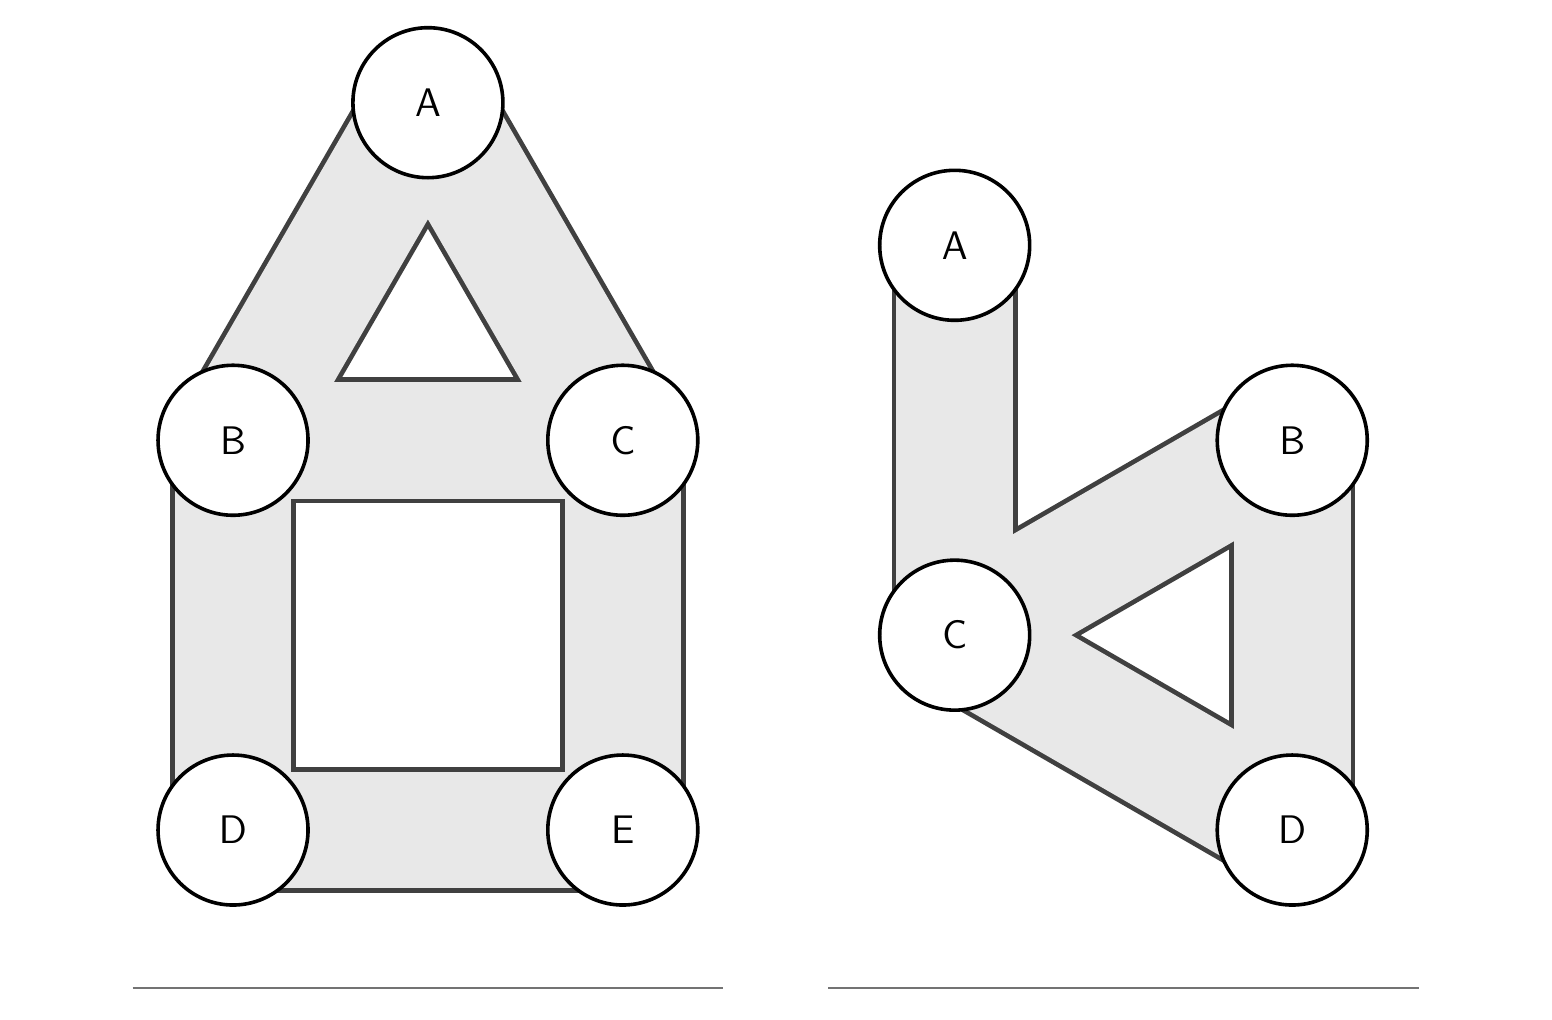
\begin{tikzpicture}
\useasboundingbox (0,0) rectangle (19.0,12.242);
\draw[bandout] (2.608,2.052) -- (7.558,2.052);
\draw[bandout] (7.558,2.052) -- (7.558,7.002);
\draw[bandout] (7.558,7.002) -- (2.608,7.002);
\draw[bandout] (2.608,7.002) -- (2.608,2.052);
\draw[bandout] (2.608,7.002) -- (5.083,11.289);
\draw[bandout] (5.083,11.289) -- (7.558,7.002);
\draw[bandfill] (2.608,2.052) -- (7.558,2.052);
\draw[bandfill] (7.558,2.052) -- (7.558,7.002);
\draw[bandfill] (7.558,7.002) -- (2.608,7.002);
\draw[bandfill] (2.608,7.002) -- (2.608,2.052);
\draw[bandfill] (2.608,7.002) -- (5.083,11.289);
\draw[bandfill] (5.083,11.289) -- (7.558,7.002);
\draw[island] (2.608,2.052) circle (0.9525);
\node[islandlabel] at (2.608,2.052) {D};
\draw[island] (7.558,2.052) circle (0.9525);
\node[islandlabel] at (7.558,2.052) {E};
\draw[island] (7.558,7.002) circle (0.9525);
\node[islandlabel] at (7.558,7.002) {C};
\draw[island] (2.608,7.002) circle (0.9525);
\node[islandlabel] at (2.608,7.002) {B};
\draw[island] (5.083,11.289) circle (0.9525);
\node[islandlabel] at (5.083,11.289) {A};
\draw[black!55, line width=0.6pt] (1.333,0.050) -- ++(7.5,0);
\draw[bandout] (16.060,2.052) -- (16.060,7.002);
\draw[bandout] (16.060,7.002) -- (11.773,4.527);
\draw[bandout] (11.773,4.527) -- (16.060,2.052);
\draw[bandout] (11.773,4.527) -- (11.773,9.478);
\draw[bandfill] (16.060,2.052) -- (16.060,7.002);
\draw[bandfill] (16.060,7.002) -- (11.773,4.527);
\draw[bandfill] (11.773,4.527) -- (16.060,2.052);
\draw[bandfill] (11.773,4.527) -- (11.773,9.478);
\draw[island] (16.060,2.052) circle (0.9525);
\node[islandlabel] at (16.060,2.052) {D};
\draw[island] (16.060,7.002) circle (0.9525);
\node[islandlabel] at (16.060,7.002) {B};
\draw[island] (11.773,4.527) circle (0.9525);
\node[islandlabel] at (11.773,4.527) {C};
\draw[island] (11.773,9.478) circle (0.9525);
\node[islandlabel] at (11.773,9.478) {A};
\draw[black!55, line width=0.6pt] (10.167,0.050) -- ++(7.5,0);
\end{tikzpicture}
\end{minipage}


\par\vspace{7mm}\noindent 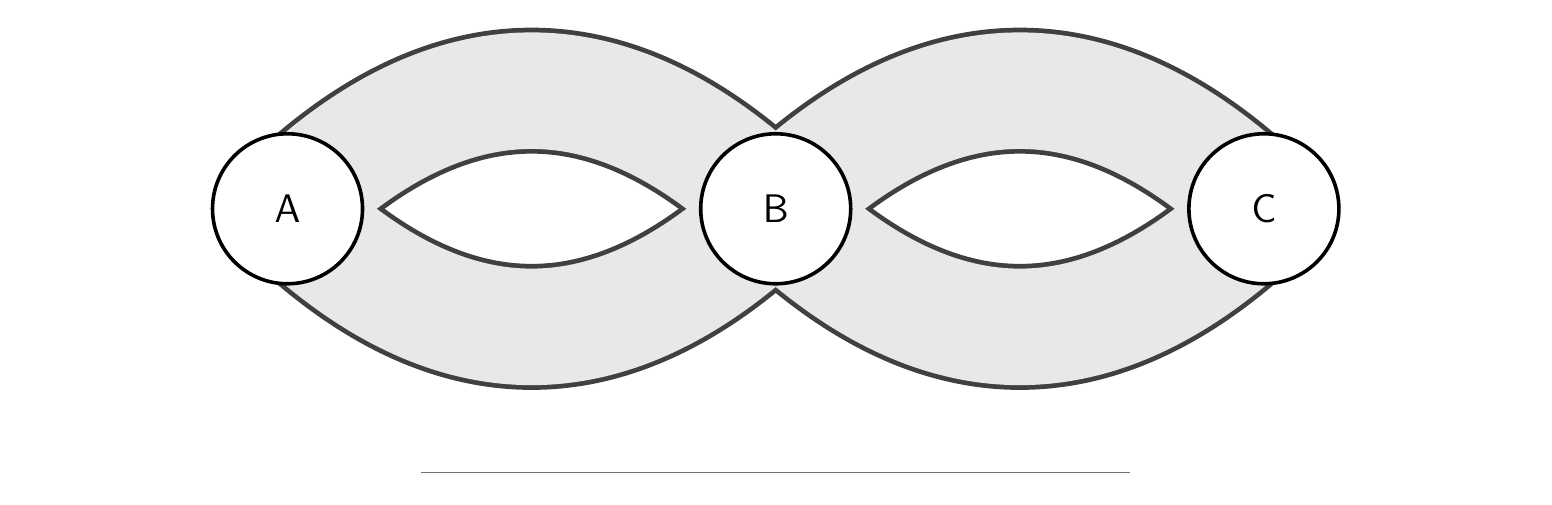
\begin{tikzpicture}
\useasboundingbox (0,0) rectangle (19.0,5.700);
\draw[bandout] (3.300,3.400) .. controls (5.367,5.400) and (7.433,5.400) .. (9.500,3.400);
\draw[bandout] (3.300,3.400) .. controls (5.367,1.400) and (7.433,1.400) .. (9.500,3.400);
\draw[bandout] (9.500,3.400) .. controls (11.567,5.400) and (13.633,5.400) .. (15.700,3.400);
\draw[bandout] (9.500,3.400) .. controls (11.567,1.400) and (13.633,1.400) .. (15.700,3.400);
\draw[bandfill] (3.300,3.400) .. controls (5.367,5.400) and (7.433,5.400) .. (9.500,3.400);
\draw[bandfill] (3.300,3.400) .. controls (5.367,1.400) and (7.433,1.400) .. (9.500,3.400);
\draw[bandfill] (9.500,3.400) .. controls (11.567,5.400) and (13.633,5.400) .. (15.700,3.400);
\draw[bandfill] (9.500,3.400) .. controls (11.567,1.400) and (13.633,1.400) .. (15.700,3.400);
\draw[island] (3.300,3.400) circle (0.9525);
\node[islandlabel] at (3.300,3.400) {A};
\draw[island] (9.500,3.400) circle (0.9525);
\node[islandlabel] at (9.500,3.400) {B};
\draw[island] (15.700,3.400) circle (0.9525);
\node[islandlabel] at (15.700,3.400) {C};
\draw[black!55, line width=0.6pt] (5.000,0.050) -- ++(9.0,0);
\end{tikzpicture}


\par\vspace{9mm}

\begin{minipage}{\linewidth}\raggedright
\prob{2}In each town, find every island where a walk that crosses every bridge exactly once can start, and where such a walk can end. If a town has no such walk, write ``none''.

\vspace{5mm}\noindent 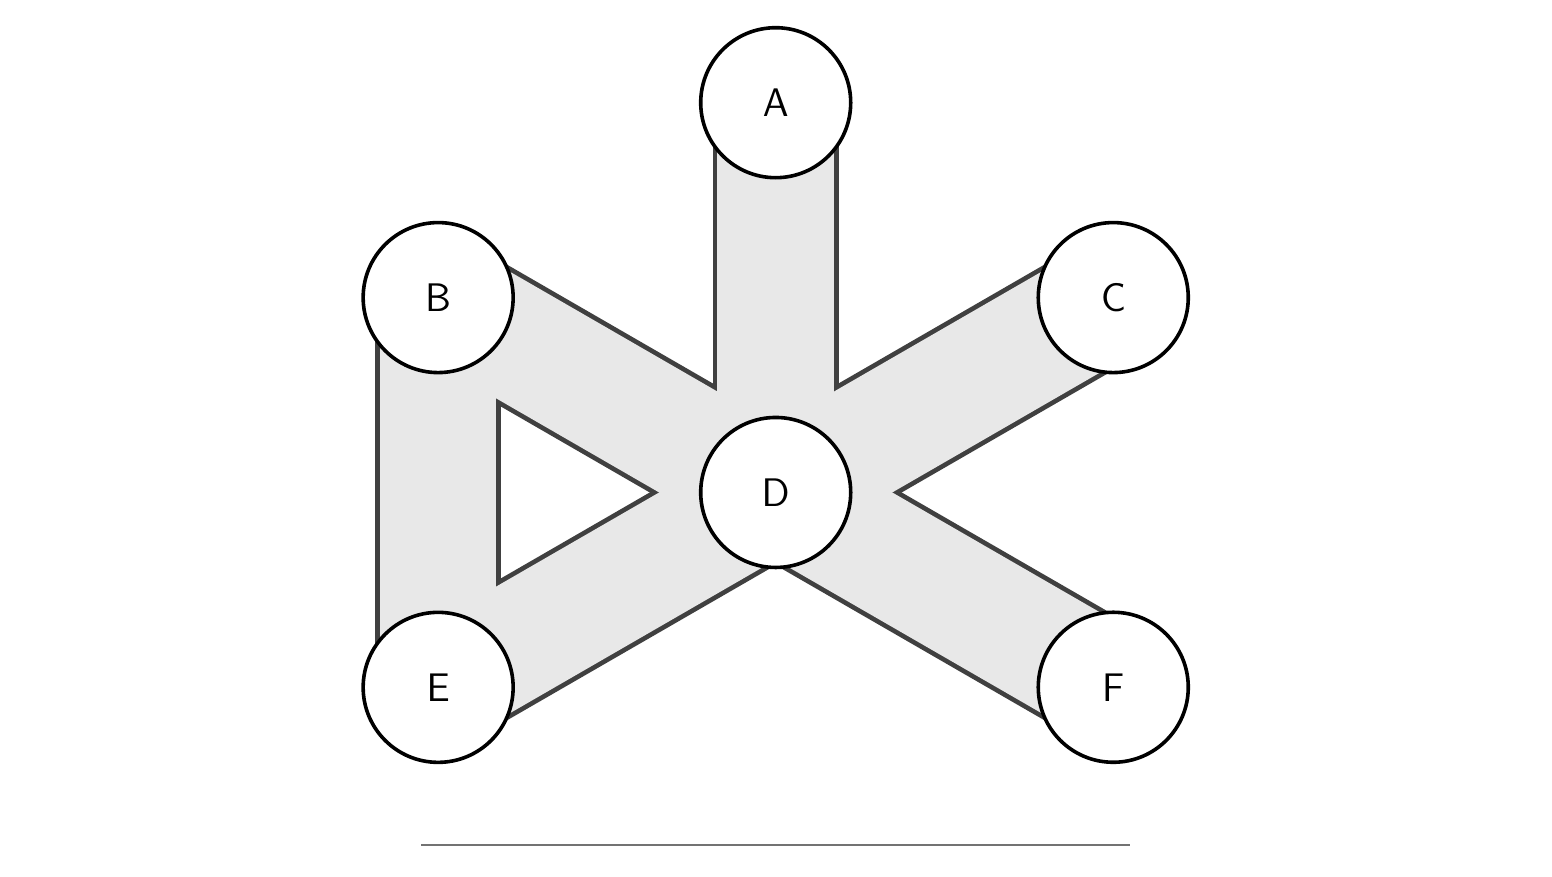
\begin{tikzpicture}
\useasboundingbox (0,0) rectangle (19.0,10.430);
\draw[bandout] (9.500,4.527) -- (5.213,2.052);
\draw[bandout] (9.500,4.527) -- (5.213,7.002);
\draw[bandout] (9.500,4.527) -- (13.787,7.002);
\draw[bandout] (9.500,4.527) -- (13.787,2.053);
\draw[bandout] (9.500,4.527) -- (9.500,9.477);
\draw[bandout] (5.213,2.052) -- (5.213,7.002);
\draw[bandfill] (9.500,4.527) -- (5.213,2.052);
\draw[bandfill] (9.500,4.527) -- (5.213,7.002);
\draw[bandfill] (9.500,4.527) -- (13.787,7.002);
\draw[bandfill] (9.500,4.527) -- (13.787,2.053);
\draw[bandfill] (9.500,4.527) -- (9.500,9.477);
\draw[bandfill] (5.213,2.052) -- (5.213,7.002);
\draw[island] (9.500,4.527) circle (0.9525);
\node[islandlabel] at (9.500,4.527) {D};
\draw[island] (5.213,2.052) circle (0.9525);
\node[islandlabel] at (5.213,2.052) {E};
\draw[island] (5.213,7.002) circle (0.9525);
\node[islandlabel] at (5.213,7.002) {B};
\draw[island] (13.787,7.002) circle (0.9525);
\node[islandlabel] at (13.787,7.002) {C};
\draw[island] (13.787,2.053) circle (0.9525);
\node[islandlabel] at (13.787,2.053) {F};
\draw[island] (9.500,9.477) circle (0.9525);
\node[islandlabel] at (9.500,9.477) {A};
\draw[black!55, line width=0.6pt] (5.000,0.050) -- ++(9.0,0);
\end{tikzpicture}
\end{minipage}


\par\vspace{7mm}\noindent 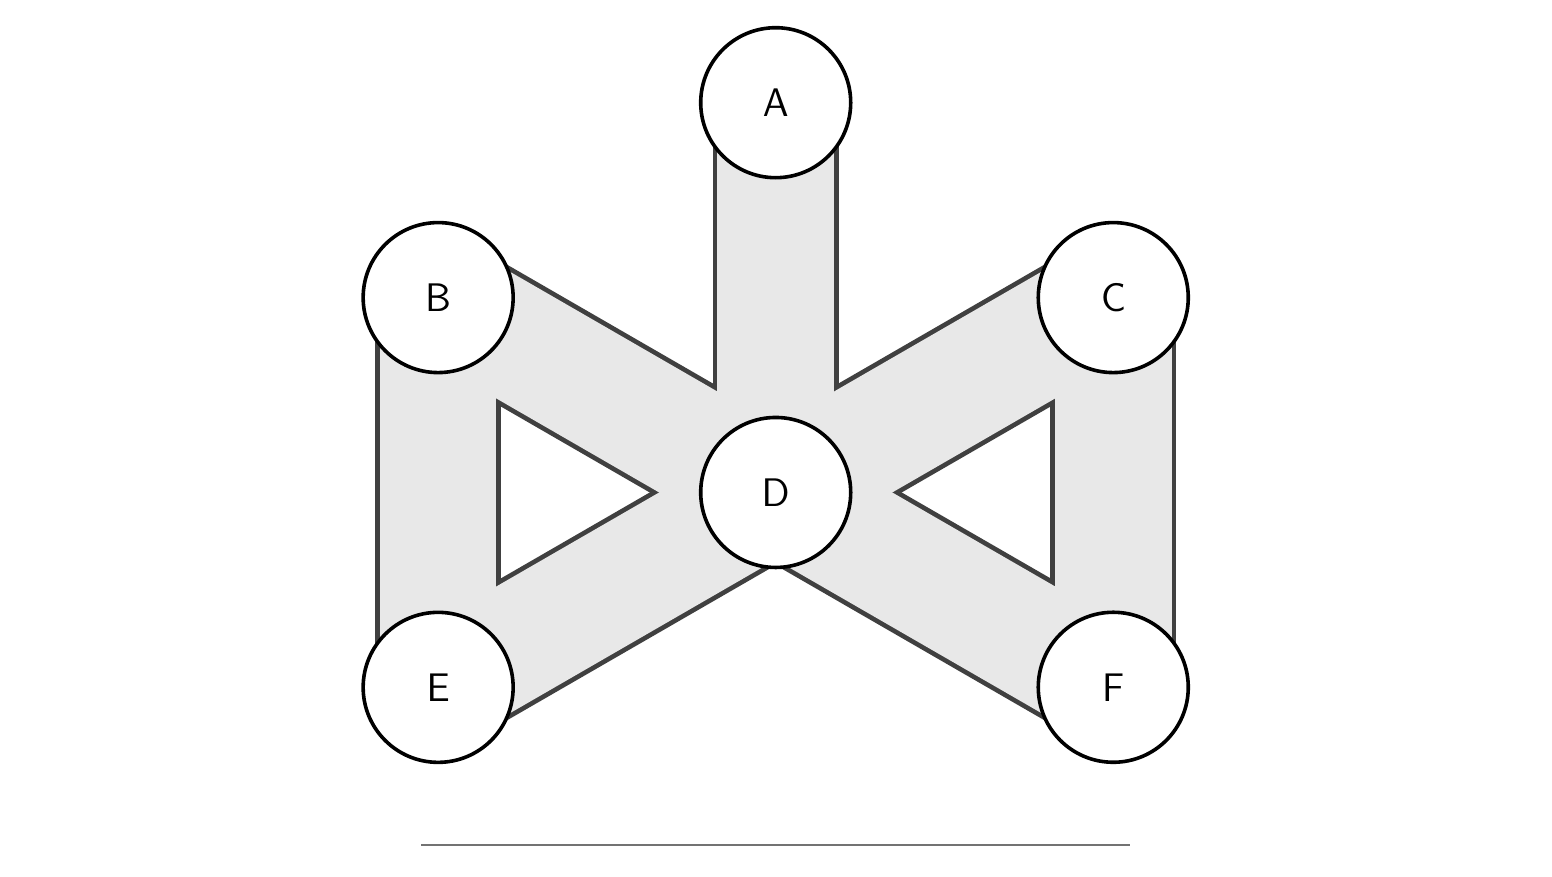
\begin{tikzpicture}
\useasboundingbox (0,0) rectangle (19.0,10.430);
\draw[bandout] (9.500,4.527) -- (5.213,2.052);
\draw[bandout] (9.500,4.527) -- (5.213,7.002);
\draw[bandout] (9.500,4.527) -- (13.787,7.002);
\draw[bandout] (9.500,4.527) -- (13.787,2.053);
\draw[bandout] (9.500,4.527) -- (9.500,9.477);
\draw[bandout] (5.213,2.052) -- (5.213,7.002);
\draw[bandout] (13.787,7.002) -- (13.787,2.053);
\draw[bandfill] (9.500,4.527) -- (5.213,2.052);
\draw[bandfill] (9.500,4.527) -- (5.213,7.002);
\draw[bandfill] (9.500,4.527) -- (13.787,7.002);
\draw[bandfill] (9.500,4.527) -- (13.787,2.053);
\draw[bandfill] (9.500,4.527) -- (9.500,9.477);
\draw[bandfill] (5.213,2.052) -- (5.213,7.002);
\draw[bandfill] (13.787,7.002) -- (13.787,2.053);
\draw[island] (9.500,4.527) circle (0.9525);
\node[islandlabel] at (9.500,4.527) {D};
\draw[island] (5.213,2.052) circle (0.9525);
\node[islandlabel] at (5.213,2.052) {E};
\draw[island] (5.213,7.002) circle (0.9525);
\node[islandlabel] at (5.213,7.002) {B};
\draw[island] (13.787,7.002) circle (0.9525);
\node[islandlabel] at (13.787,7.002) {C};
\draw[island] (13.787,2.053) circle (0.9525);
\node[islandlabel] at (13.787,2.053) {F};
\draw[island] (9.500,9.477) circle (0.9525);
\node[islandlabel] at (9.500,9.477) {A};
\draw[black!55, line width=0.6pt] (5.000,0.050) -- ++(9.0,0);
\end{tikzpicture}


\par\vspace{7mm}\noindent 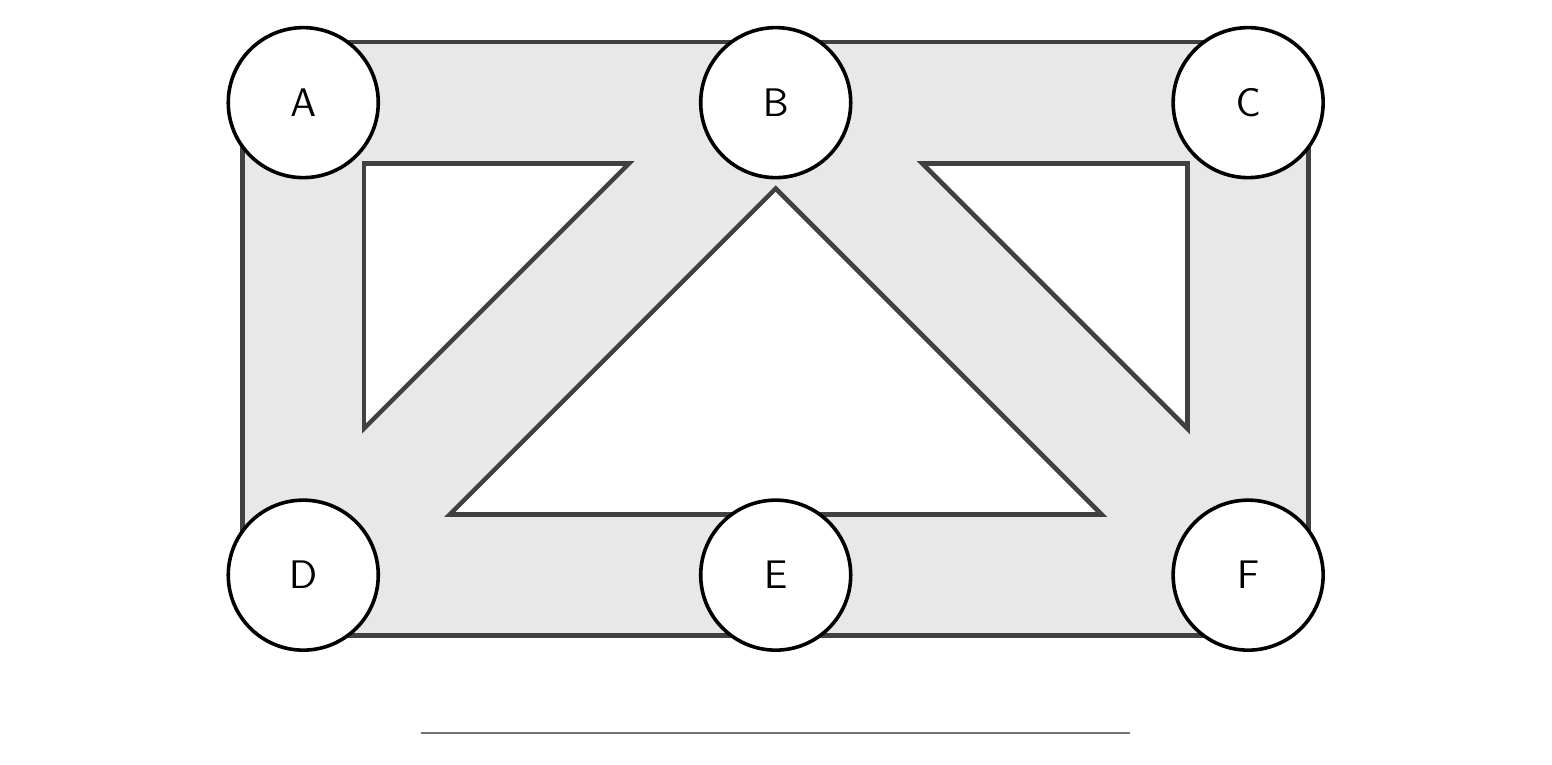
\begin{tikzpicture}
\useasboundingbox (0,0) rectangle (19.0,9.005);
\draw[bandout] (3.500,2.052) -- (9.500,2.052);
\draw[bandout] (9.500,2.052) -- (15.500,2.052);
\draw[bandout] (3.500,8.053) -- (9.500,8.053);
\draw[bandout] (9.500,8.053) -- (15.500,8.053);
\draw[bandout] (3.500,2.052) -- (3.500,8.053);
\draw[bandout] (15.500,2.052) -- (15.500,8.053);
\draw[bandout] (9.500,8.053) -- (3.500,2.052);
\draw[bandout] (9.500,8.053) -- (15.500,2.052);
\draw[bandfill] (3.500,2.052) -- (9.500,2.052);
\draw[bandfill] (9.500,2.052) -- (15.500,2.052);
\draw[bandfill] (3.500,8.053) -- (9.500,8.053);
\draw[bandfill] (9.500,8.053) -- (15.500,8.053);
\draw[bandfill] (3.500,2.052) -- (3.500,8.053);
\draw[bandfill] (15.500,2.052) -- (15.500,8.053);
\draw[bandfill] (9.500,8.053) -- (3.500,2.052);
\draw[bandfill] (9.500,8.053) -- (15.500,2.052);
\draw[island] (3.500,2.052) circle (0.9525);
\node[islandlabel] at (3.500,2.052) {D};
\draw[island] (3.500,8.053) circle (0.9525);
\node[islandlabel] at (3.500,8.053) {A};
\draw[island] (9.500,2.052) circle (0.9525);
\node[islandlabel] at (9.500,2.052) {E};
\draw[island] (9.500,8.053) circle (0.9525);
\node[islandlabel] at (9.500,8.053) {B};
\draw[island] (15.500,2.052) circle (0.9525);
\node[islandlabel] at (15.500,2.052) {F};
\draw[island] (15.500,8.053) circle (0.9525);
\node[islandlabel] at (15.500,8.053) {C};
\draw[black!55, line width=0.6pt] (5.000,0.050) -- ++(9.0,0);
\end{tikzpicture}


\par\vspace{7mm}\noindent 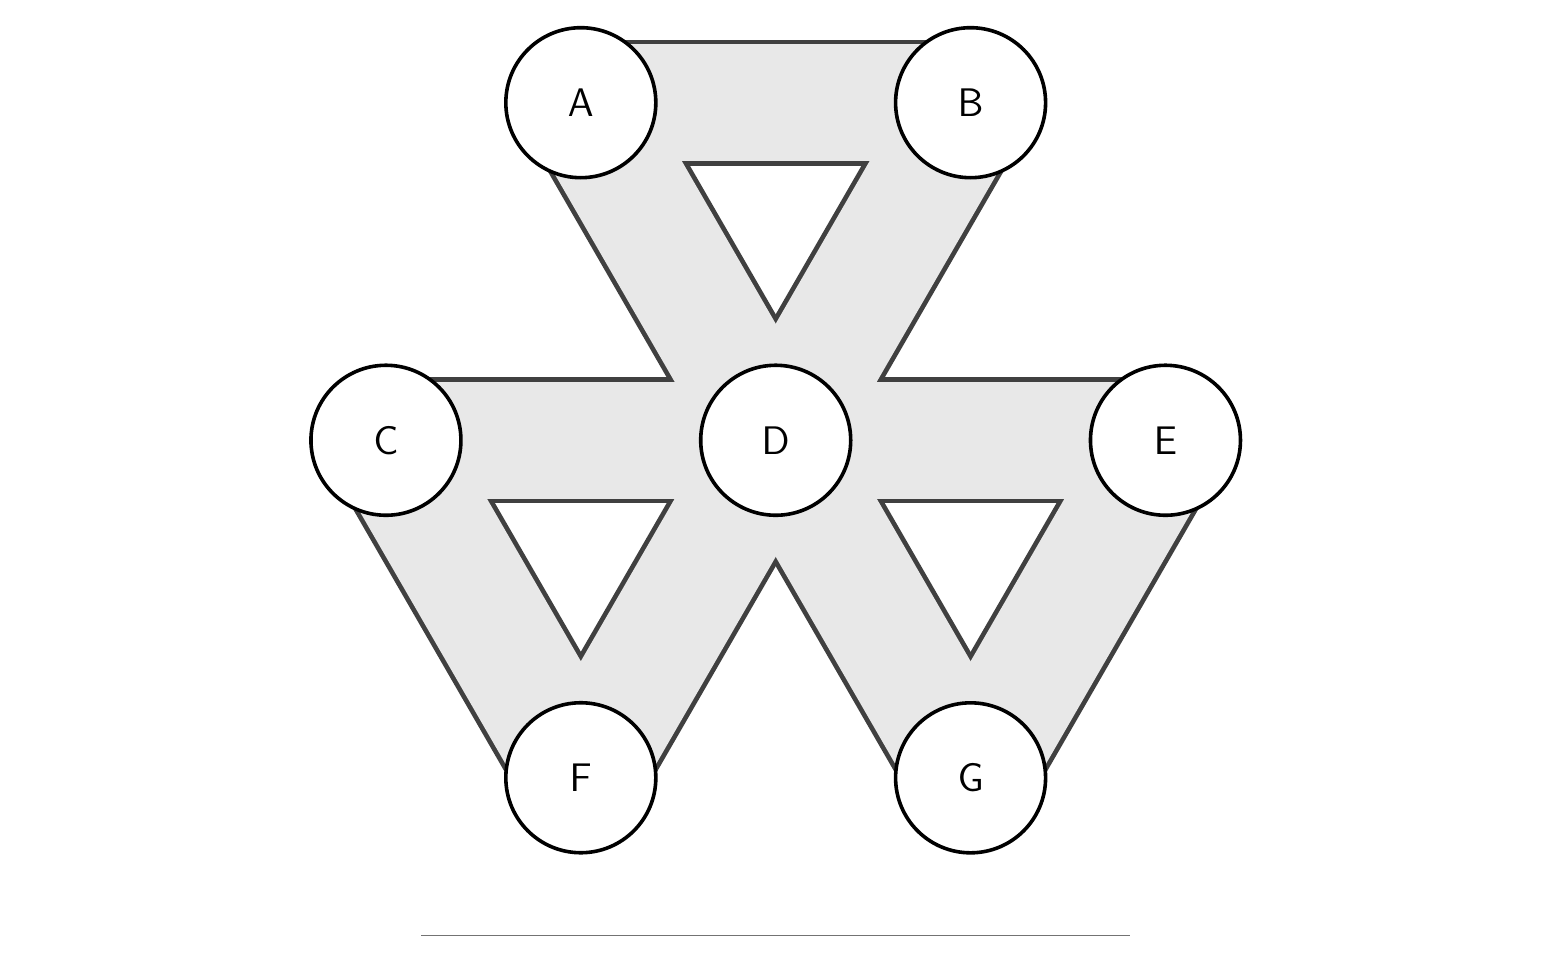
\begin{tikzpicture}
\useasboundingbox (0,0) rectangle (19.0,11.579);
\draw[bandout] (9.500,6.339) -- (11.975,10.626);
\draw[bandout] (11.975,10.626) -- (7.025,10.626);
\draw[bandout] (7.025,10.626) -- (9.500,6.339);
\draw[bandout] (9.500,6.339) -- (4.550,6.339);
\draw[bandout] (4.550,6.339) -- (7.025,2.053);
\draw[bandout] (7.025,2.053) -- (9.500,6.339);
\draw[bandout] (9.500,6.339) -- (11.975,2.052);
\draw[bandout] (11.975,2.052) -- (14.450,6.339);
\draw[bandout] (14.450,6.339) -- (9.500,6.339);
\draw[bandfill] (9.500,6.339) -- (11.975,10.626);
\draw[bandfill] (11.975,10.626) -- (7.025,10.626);
\draw[bandfill] (7.025,10.626) -- (9.500,6.339);
\draw[bandfill] (9.500,6.339) -- (4.550,6.339);
\draw[bandfill] (4.550,6.339) -- (7.025,2.053);
\draw[bandfill] (7.025,2.053) -- (9.500,6.339);
\draw[bandfill] (9.500,6.339) -- (11.975,2.052);
\draw[bandfill] (11.975,2.052) -- (14.450,6.339);
\draw[bandfill] (14.450,6.339) -- (9.500,6.339);
\draw[island] (9.500,6.339) circle (0.9525);
\node[islandlabel] at (9.500,6.339) {D};
\draw[island] (11.975,10.626) circle (0.9525);
\node[islandlabel] at (11.975,10.626) {B};
\draw[island] (7.025,10.626) circle (0.9525);
\node[islandlabel] at (7.025,10.626) {A};
\draw[island] (4.550,6.339) circle (0.9525);
\node[islandlabel] at (4.550,6.339) {C};
\draw[island] (7.025,2.053) circle (0.9525);
\node[islandlabel] at (7.025,2.053) {F};
\draw[island] (11.975,2.052) circle (0.9525);
\node[islandlabel] at (11.975,2.052) {G};
\draw[island] (14.450,6.339) circle (0.9525);
\node[islandlabel] at (14.450,6.339) {E};
\draw[black!55, line width=0.6pt] (5.000,0.050) -- ++(9.0,0);
\end{tikzpicture}


\par\vspace{9mm}

\begin{minipage}{\linewidth}\raggedright
\prob{3}For each town, decide without walking it whether there is a walk that crosses every bridge exactly once, and if there is, where it can start and end. If there is none, write ``none''. Then use counters to check each town that has a walk.

\vspace{5mm}\noindent 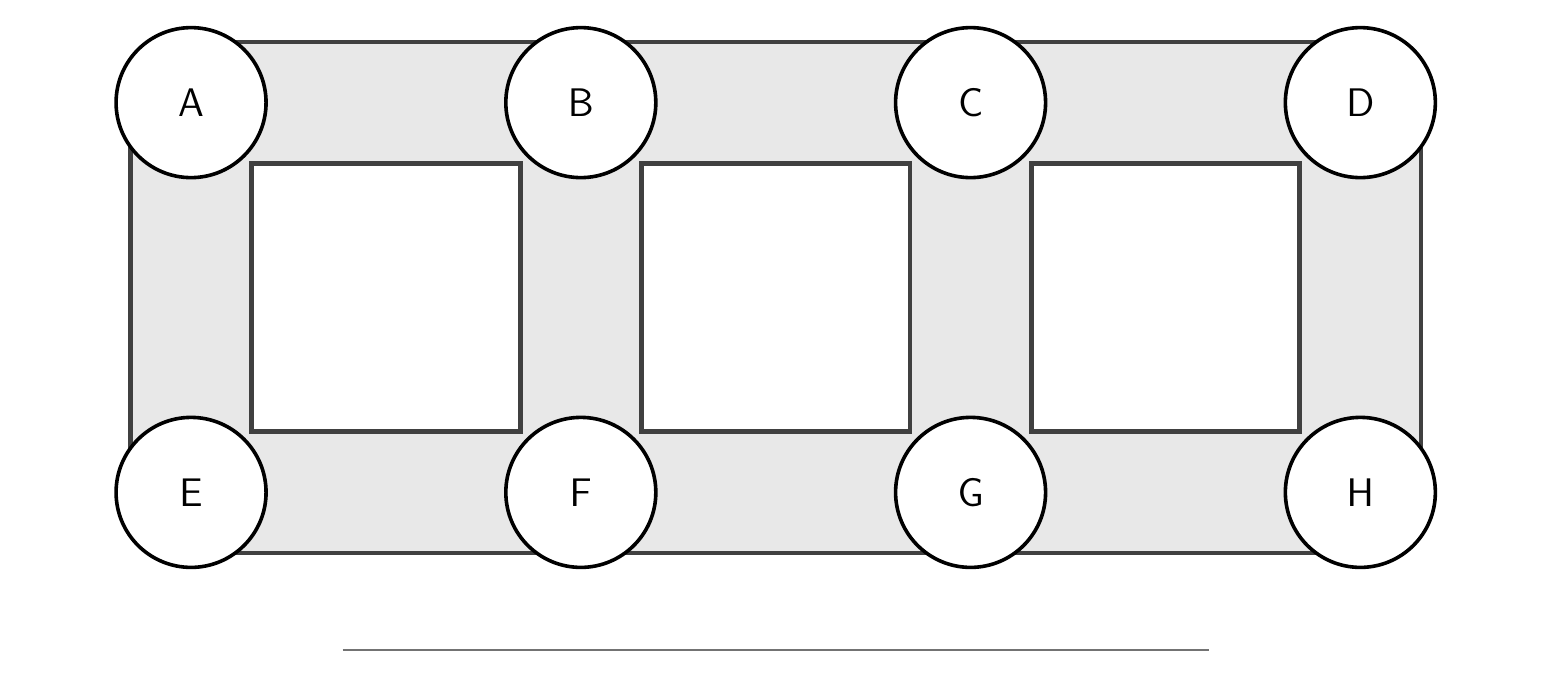
\begin{tikzpicture}
\useasboundingbox (0,0) rectangle (19.0,7.955);
\draw[bandout] (2.075,2.053) -- (7.025,2.053);
\draw[bandout] (2.075,7.003) -- (7.025,7.003);
\draw[bandout] (7.025,2.053) -- (11.975,2.053);
\draw[bandout] (7.025,7.003) -- (11.975,7.003);
\draw[bandout] (11.975,2.053) -- (16.925,2.053);
\draw[bandout] (11.975,7.003) -- (16.925,7.003);
\draw[bandout] (2.075,2.053) -- (2.075,7.003);
\draw[bandout] (7.025,2.053) -- (7.025,7.003);
\draw[bandout] (11.975,2.053) -- (11.975,7.003);
\draw[bandout] (16.925,2.053) -- (16.925,7.003);
\draw[bandfill] (2.075,2.053) -- (7.025,2.053);
\draw[bandfill] (2.075,7.003) -- (7.025,7.003);
\draw[bandfill] (7.025,2.053) -- (11.975,2.053);
\draw[bandfill] (7.025,7.003) -- (11.975,7.003);
\draw[bandfill] (11.975,2.053) -- (16.925,2.053);
\draw[bandfill] (11.975,7.003) -- (16.925,7.003);
\draw[bandfill] (2.075,2.053) -- (2.075,7.003);
\draw[bandfill] (7.025,2.053) -- (7.025,7.003);
\draw[bandfill] (11.975,2.053) -- (11.975,7.003);
\draw[bandfill] (16.925,2.053) -- (16.925,7.003);
\draw[island] (2.075,2.053) circle (0.9525);
\node[islandlabel] at (2.075,2.053) {E};
\draw[island] (7.025,2.053) circle (0.9525);
\node[islandlabel] at (7.025,2.053) {F};
\draw[island] (11.975,2.053) circle (0.9525);
\node[islandlabel] at (11.975,2.053) {G};
\draw[island] (16.925,2.053) circle (0.9525);
\node[islandlabel] at (16.925,2.053) {H};
\draw[island] (2.075,7.003) circle (0.9525);
\node[islandlabel] at (2.075,7.003) {A};
\draw[island] (7.025,7.003) circle (0.9525);
\node[islandlabel] at (7.025,7.003) {B};
\draw[island] (11.975,7.003) circle (0.9525);
\node[islandlabel] at (11.975,7.003) {C};
\draw[island] (16.925,7.003) circle (0.9525);
\node[islandlabel] at (16.925,7.003) {D};
\draw[black!55, line width=0.6pt] (4.000,0.050) -- ++(11.0,0);
\end{tikzpicture}
\end{minipage}


\par\vspace{7mm}\noindent 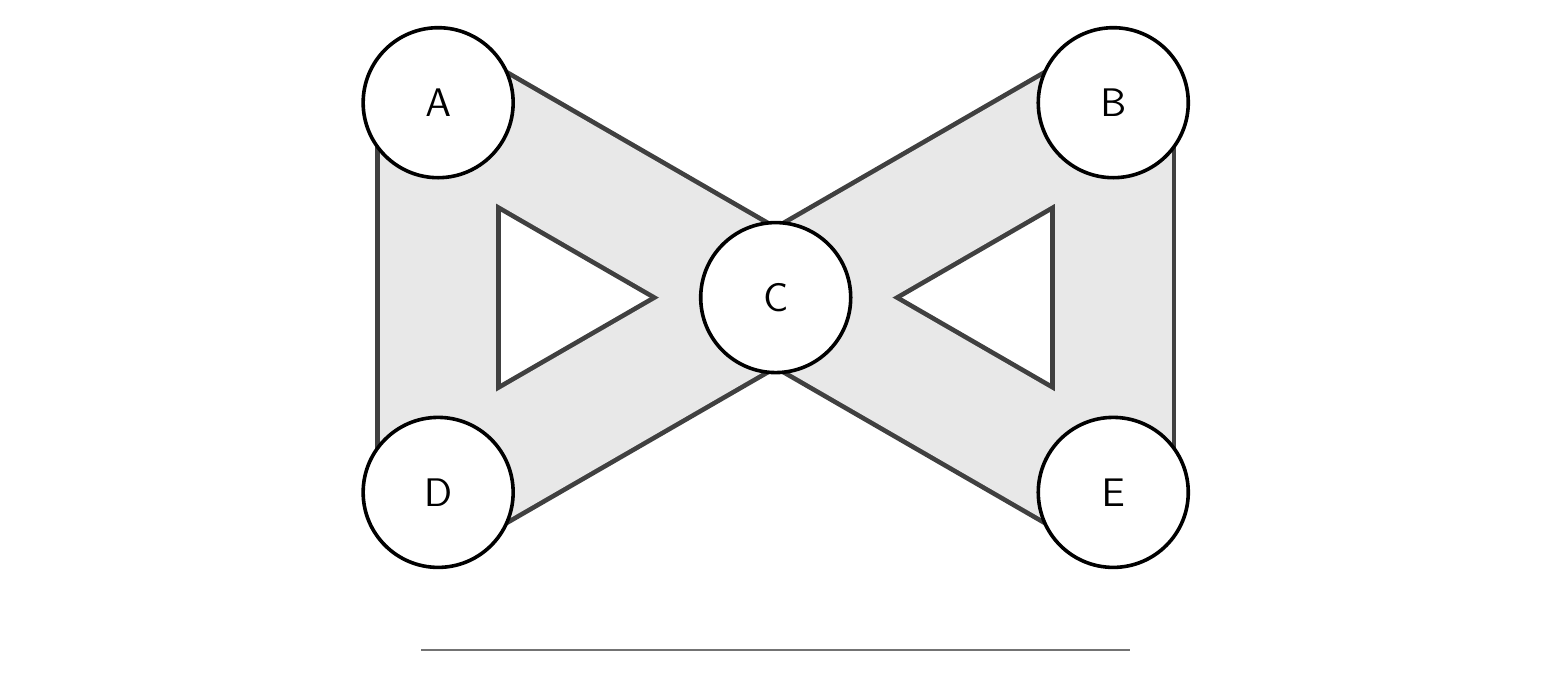
\begin{tikzpicture}
\useasboundingbox (0,0) rectangle (19.0,7.955);
\draw[bandout] (9.500,4.527) -- (5.213,7.002);
\draw[bandout] (5.213,7.002) -- (5.213,2.053);
\draw[bandout] (5.213,2.053) -- (9.500,4.527);
\draw[bandout] (9.500,4.527) -- (13.787,7.002);
\draw[bandout] (13.787,7.002) -- (13.787,2.053);
\draw[bandout] (13.787,2.053) -- (9.500,4.527);
\draw[bandfill] (9.500,4.527) -- (5.213,7.002);
\draw[bandfill] (5.213,7.002) -- (5.213,2.053);
\draw[bandfill] (5.213,2.053) -- (9.500,4.527);
\draw[bandfill] (9.500,4.527) -- (13.787,7.002);
\draw[bandfill] (13.787,7.002) -- (13.787,2.053);
\draw[bandfill] (13.787,2.053) -- (9.500,4.527);
\draw[island] (5.213,7.002) circle (0.9525);
\node[islandlabel] at (5.213,7.002) {A};
\draw[island] (5.213,2.053) circle (0.9525);
\node[islandlabel] at (5.213,2.053) {D};
\draw[island] (9.500,4.527) circle (0.9525);
\node[islandlabel] at (9.500,4.527) {C};
\draw[island] (13.787,7.002) circle (0.9525);
\node[islandlabel] at (13.787,7.002) {B};
\draw[island] (13.787,2.053) circle (0.9525);
\node[islandlabel] at (13.787,2.053) {E};
\draw[black!55, line width=0.6pt] (5.000,0.050) -- ++(9.0,0);
\end{tikzpicture}


\par\vspace{7mm}\noindent 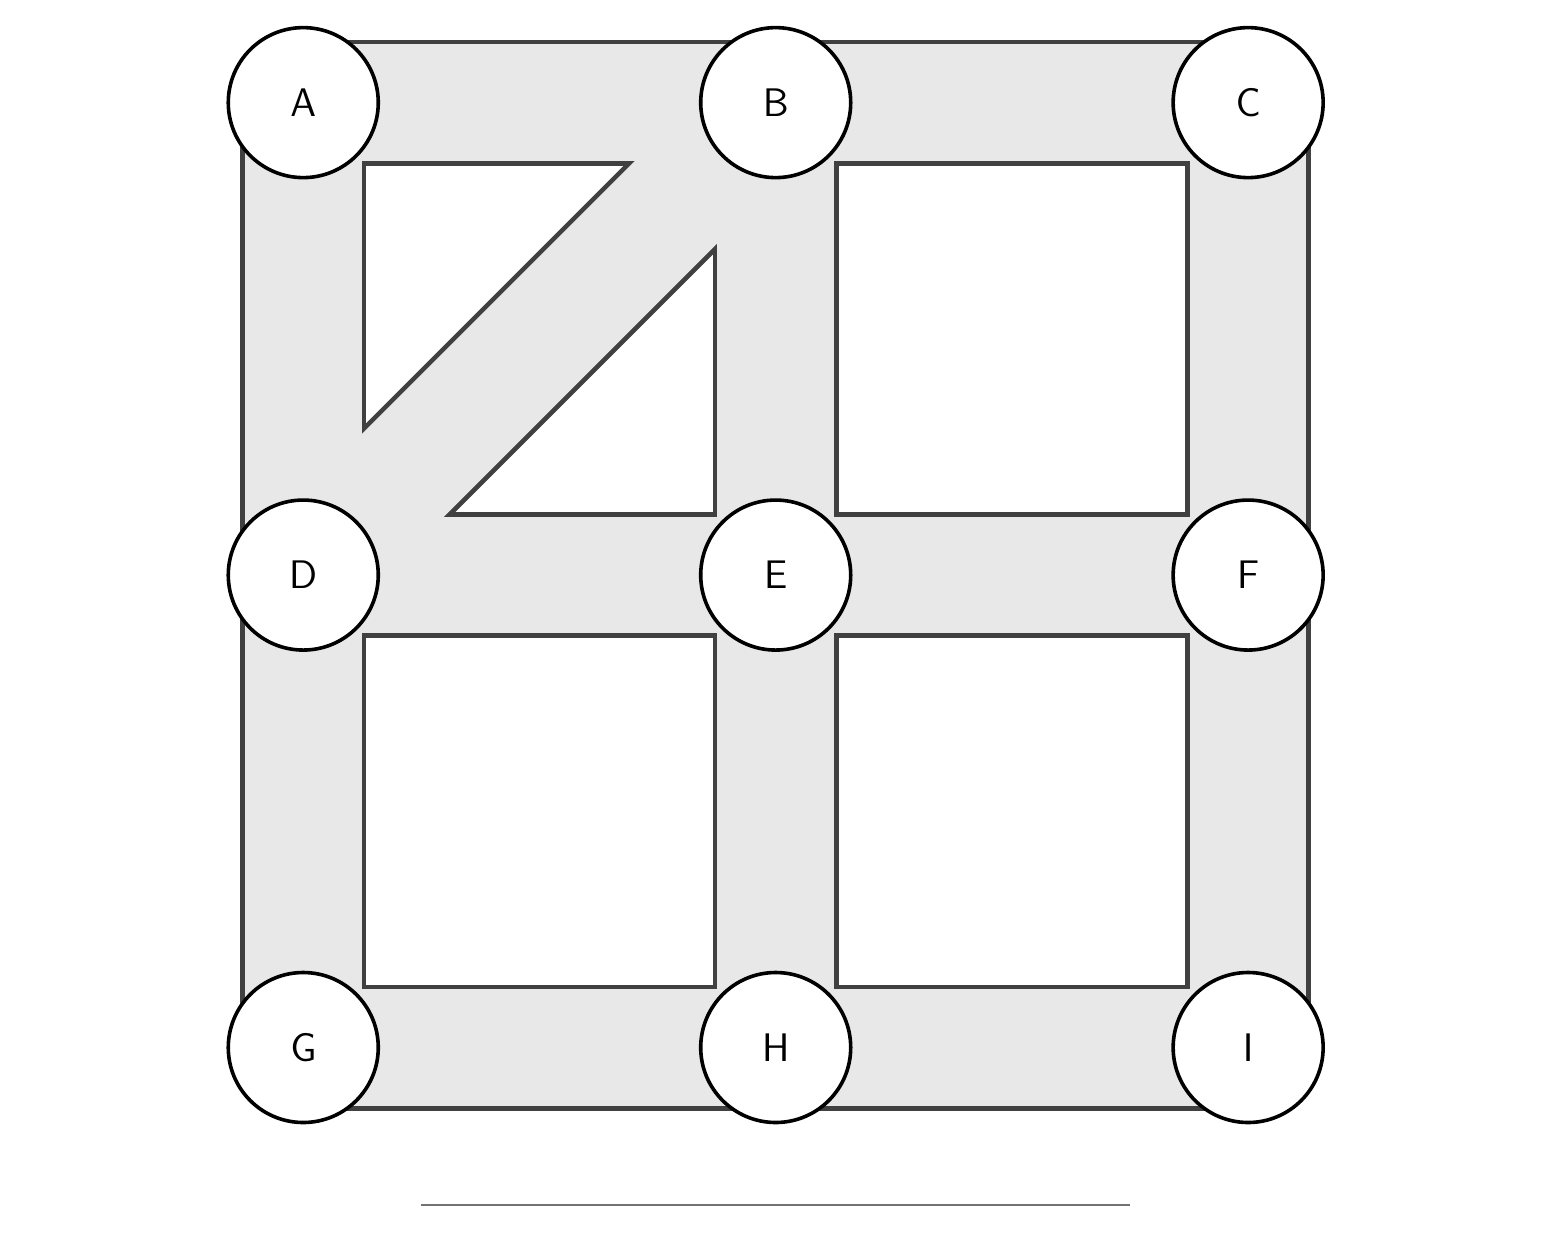
\begin{tikzpicture}
\useasboundingbox (0,0) rectangle (19.0,15.005);
\draw[bandout] (3.500,14.053) -- (9.500,14.053);
\draw[bandout] (3.500,14.053) -- (3.500,8.053);
\draw[bandout] (9.500,14.053) -- (15.500,14.053);
\draw[bandout] (9.500,14.053) -- (9.500,8.053);
\draw[bandout] (15.500,14.053) -- (15.500,8.053);
\draw[bandout] (3.500,8.053) -- (9.500,8.053);
\draw[bandout] (3.500,8.053) -- (3.500,2.053);
\draw[bandout] (9.500,8.053) -- (15.500,8.053);
\draw[bandout] (9.500,8.053) -- (9.500,2.053);
\draw[bandout] (15.500,8.053) -- (15.500,2.053);
\draw[bandout] (3.500,2.053) -- (9.500,2.053);
\draw[bandout] (9.500,2.053) -- (15.500,2.053);
\draw[bandout] (9.500,14.053) -- (3.500,8.053);
\draw[bandfill] (3.500,14.053) -- (9.500,14.053);
\draw[bandfill] (3.500,14.053) -- (3.500,8.053);
\draw[bandfill] (9.500,14.053) -- (15.500,14.053);
\draw[bandfill] (9.500,14.053) -- (9.500,8.053);
\draw[bandfill] (15.500,14.053) -- (15.500,8.053);
\draw[bandfill] (3.500,8.053) -- (9.500,8.053);
\draw[bandfill] (3.500,8.053) -- (3.500,2.053);
\draw[bandfill] (9.500,8.053) -- (15.500,8.053);
\draw[bandfill] (9.500,8.053) -- (9.500,2.053);
\draw[bandfill] (15.500,8.053) -- (15.500,2.053);
\draw[bandfill] (3.500,2.053) -- (9.500,2.053);
\draw[bandfill] (9.500,2.053) -- (15.500,2.053);
\draw[bandfill] (9.500,14.053) -- (3.500,8.053);
\draw[island] (3.500,14.053) circle (0.9525);
\node[islandlabel] at (3.500,14.053) {A};
\draw[island] (9.500,14.053) circle (0.9525);
\node[islandlabel] at (9.500,14.053) {B};
\draw[island] (15.500,14.053) circle (0.9525);
\node[islandlabel] at (15.500,14.053) {C};
\draw[island] (3.500,8.053) circle (0.9525);
\node[islandlabel] at (3.500,8.053) {D};
\draw[island] (9.500,8.053) circle (0.9525);
\node[islandlabel] at (9.500,8.053) {E};
\draw[island] (15.500,8.053) circle (0.9525);
\node[islandlabel] at (15.500,8.053) {F};
\draw[island] (3.500,2.053) circle (0.9525);
\node[islandlabel] at (3.500,2.053) {G};
\draw[island] (9.500,2.053) circle (0.9525);
\node[islandlabel] at (9.500,2.053) {H};
\draw[island] (15.500,2.053) circle (0.9525);
\node[islandlabel] at (15.500,2.053) {I};
\draw[black!55, line width=0.6pt] (5.000,0.050) -- ++(9.0,0);
\end{tikzpicture}


\par\vspace{9mm}

\begin{minipage}{\linewidth}\raggedright
\prob{4}Write a rule that tells you, from a picture of a town, whether it has a walk that crosses every bridge exactly once, and where such a walk can start and end. Explain why a town that breaks your rule cannot have such a walk.

\vspace{5mm}\noindent \begin{tikzpicture}
\useasboundingbox (0,0) rectangle (19.0,6.000);
\draw[black!55, line width=0.6pt] (0.000,0.050) -- ++(19.0,0);
\draw[black!55, line width=0.6pt] (0.000,1.050) -- ++(19.0,0);
\draw[black!55, line width=0.6pt] (0.000,2.050) -- ++(19.0,0);
\draw[black!55, line width=0.6pt] (0.000,3.050) -- ++(19.0,0);
\draw[black!55, line width=0.6pt] (0.000,4.050) -- ++(19.0,0);
\draw[black!55, line width=0.6pt] (0.000,5.050) -- ++(19.0,0);
\end{tikzpicture}
\end{minipage}


\par\vspace{9mm}

\newpage

\begin{minipage}{\linewidth}\raggedright
\prob{5}In the city of K\"onigsberg, seven bridges joined four areas of land, A, B, C and D. Can someone walk through the city crossing every bridge exactly once? Explain. Where could the city build one new bridge so that such a walk becomes possible? What is the smallest number of new bridges the city needs for a walk that crosses every bridge exactly once and ends where it started?

\vspace{5mm}\noindent 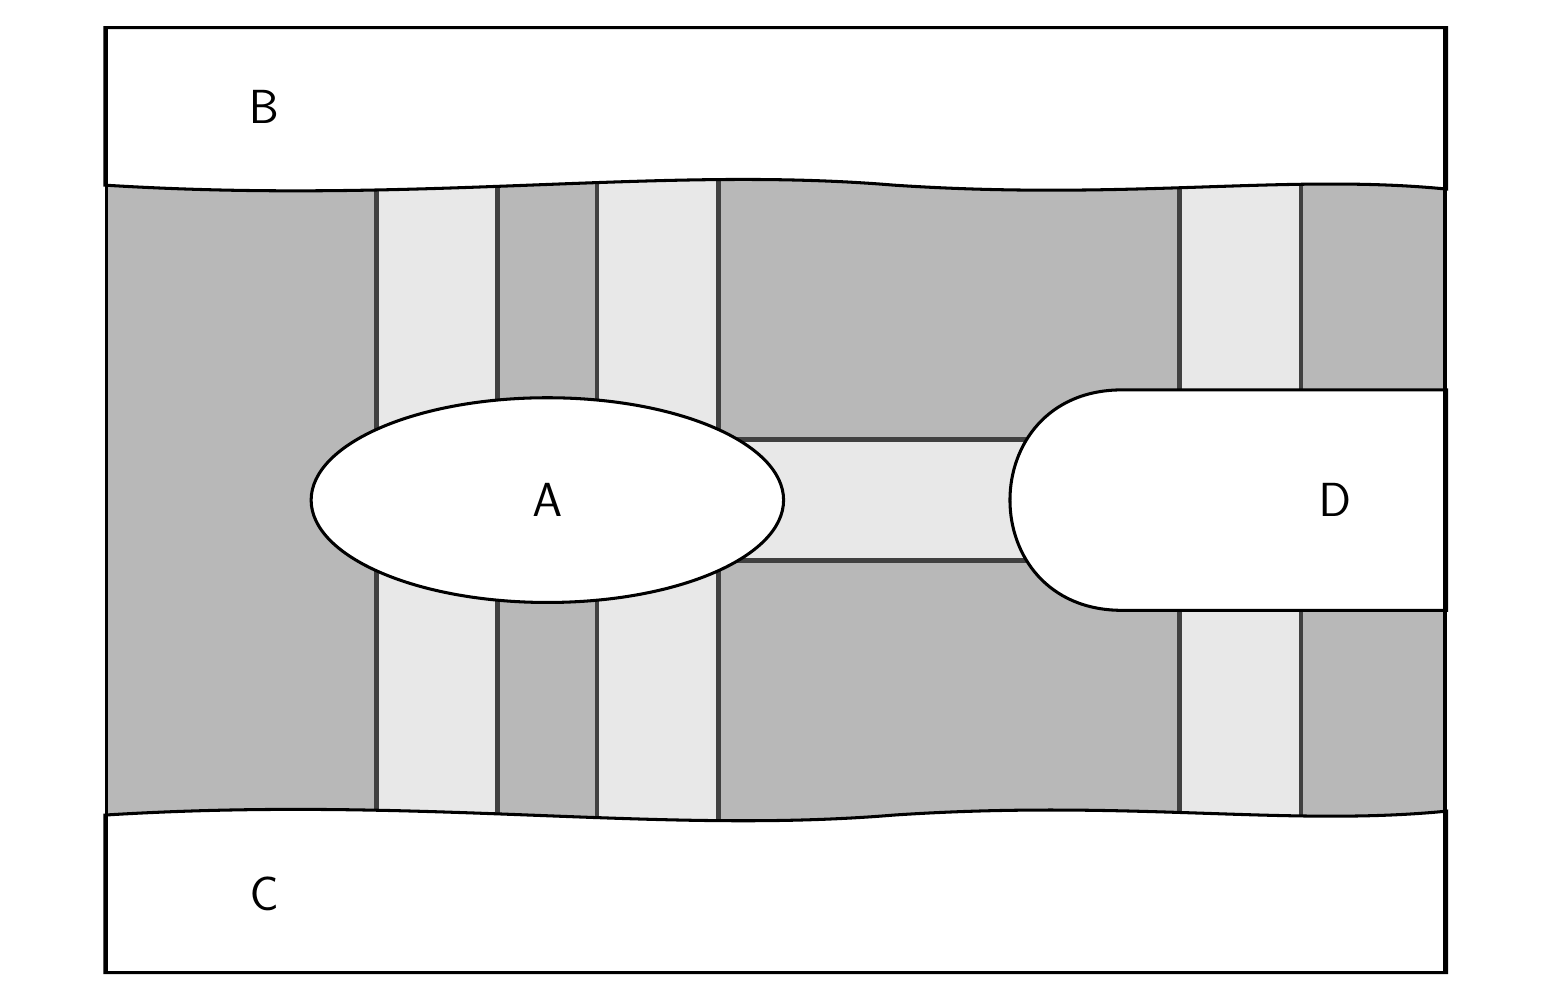
\begin{tikzpicture}
\useasboundingbox (0,0) rectangle (19.0,12.000);
\begin{scope}[shift={(1.000,0.000)}]
\fill[black!28] (0,0) rectangle (17.0,12.0);
\draw[bandout] (4.2,6.0) -- (4.2,10.4);
\draw[bandout] (7.0,6.0) -- (7.0,10.4);
\draw[bandout] (4.2,6.0) -- (4.2,1.6);
\draw[bandout] (7.0,6.0) -- (7.0,1.6);
\draw[bandout] (7.6,6.0) -- (12.2,6.0);
\draw[bandout] (14.4,6.0) -- (14.4,10.4);
\draw[bandout] (14.4,6.0) -- (14.4,1.6);
\draw[bandfill] (4.2,6.0) -- (4.2,10.4);
\draw[bandfill] (7.0,6.0) -- (7.0,10.4);
\draw[bandfill] (4.2,6.0) -- (4.2,1.6);
\draw[bandfill] (7.0,6.0) -- (7.0,1.6);
\draw[bandfill] (7.6,6.0) -- (12.2,6.0);
\draw[bandfill] (14.4,6.0) -- (14.4,10.4);
\draw[bandfill] (14.4,6.0) -- (14.4,1.6);
\filldraw[fill=white, draw=black, line width=1.1pt] (-0.02,12.0) -- (-0.02,10.0) .. controls (4,9.75) and (7,10.25) .. (10,10.0) .. controls (13,9.8) and (15,10.15) .. (17.02,9.95) -- (17.02,12.0) -- cycle;
\filldraw[fill=white, draw=black, line width=1.1pt] (-0.02,0) -- (-0.02,2.0) .. controls (4,2.25) and (7,1.75) .. (10,2.0) .. controls (13,2.2) and (15,1.85) .. (17.02,2.05) -- (17.02,0) -- cycle;
\filldraw[fill=white, draw=black, line width=1.1pt] (5.6,6.0) ellipse (3.0 and 1.3);
\filldraw[fill=white, draw=black, line width=1.1pt] (17.02,4.6) -- (12.9,4.6) .. controls (11.0,4.6) and (11.0,7.4) .. (12.9,7.4) -- (17.02,7.4) -- cycle;
\draw[line width=1.1pt] (0,0) rectangle (17.0,12.0);
\node[font=\sffamily\LARGE] at (5.6,6.0) {A};
\node[font=\sffamily\LARGE] at (2.0,11.0) {B};
\node[font=\sffamily\LARGE] at (2.0,1.0) {C};
\node[font=\sffamily\LARGE] at (15.6,6.0) {D};
\end{scope}
\end{tikzpicture}
\end{minipage}


\par\vspace{7mm}\noindent \begin{tikzpicture}
\useasboundingbox (0,0) rectangle (19.0,6.000);
\draw[black!55, line width=0.6pt] (0.000,0.050) -- ++(19.0,0);
\draw[black!55, line width=0.6pt] (0.000,1.050) -- ++(19.0,0);
\draw[black!55, line width=0.6pt] (0.000,2.050) -- ++(19.0,0);
\draw[black!55, line width=0.6pt] (0.000,3.050) -- ++(19.0,0);
\draw[black!55, line width=0.6pt] (0.000,4.050) -- ++(19.0,0);
\draw[black!55, line width=0.6pt] (0.000,5.050) -- ++(19.0,0);
\end{tikzpicture}


\par\vspace{9mm}

\begin{minipage}{\linewidth}\raggedright
\prob{6}Can a town have exactly one island with an odd number of bridges? Can it have exactly three? Explain.

\vspace{5mm}\noindent \begin{tikzpicture}
\useasboundingbox (0,0) rectangle (19.0,6.000);
\draw[black!55, line width=0.6pt] (0.000,0.050) -- ++(19.0,0);
\draw[black!55, line width=0.6pt] (0.000,1.050) -- ++(19.0,0);
\draw[black!55, line width=0.6pt] (0.000,2.050) -- ++(19.0,0);
\draw[black!55, line width=0.6pt] (0.000,3.050) -- ++(19.0,0);
\draw[black!55, line width=0.6pt] (0.000,4.050) -- ++(19.0,0);
\draw[black!55, line width=0.6pt] (0.000,5.050) -- ++(19.0,0);
\end{tikzpicture}
\end{minipage}


\par\vspace{9mm}

\begin{minipage}{\linewidth}\raggedright
\prob{7}Trace each picture with a colored pencil, without lifting the pencil and without going over a line twice, or explain why it cannot be done. For each picture that cannot be traced this way, find the fewest strokes that draw it without going over a line twice, using a new color for each stroke.

\vspace{5mm}\noindent 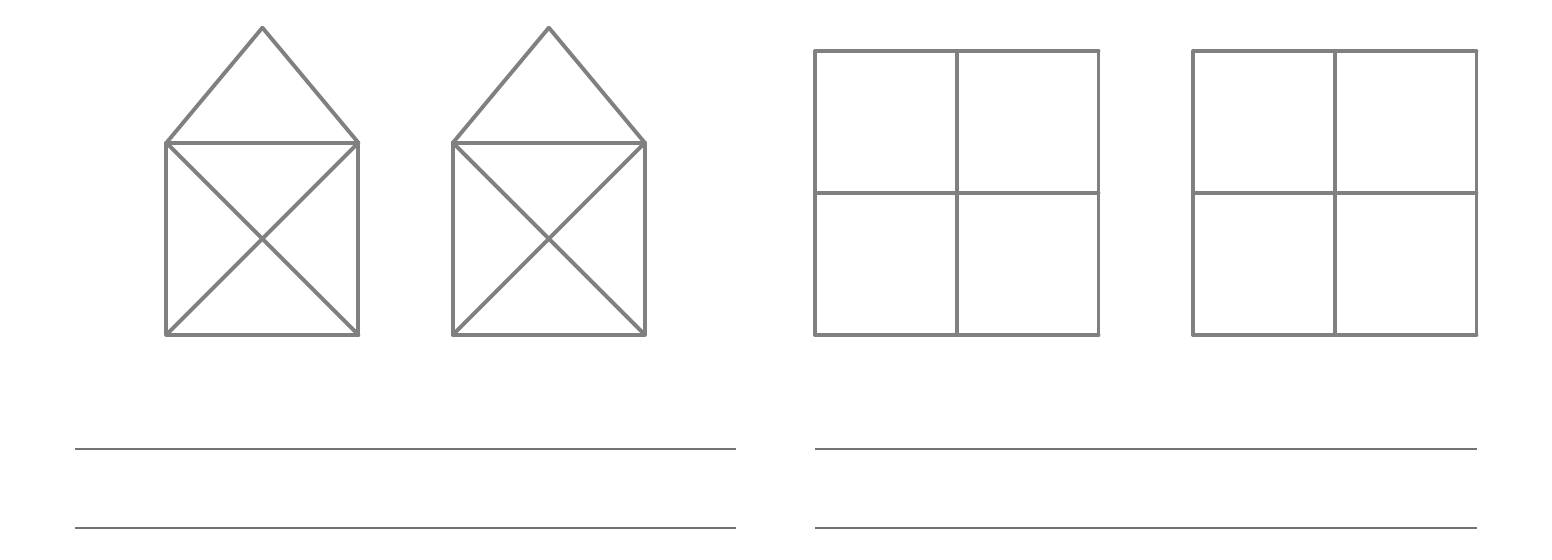
\begin{tikzpicture}
\useasboundingbox (0,0) rectangle (19.0,6.400);
\draw[stroke] (1.762,2.500) -- (4.200,2.500);
\draw[stroke] (4.200,2.500) -- (4.200,4.938);
\draw[stroke] (4.200,4.938) -- (1.762,4.938);
\draw[stroke] (1.762,4.938) -- (1.762,2.500);
\draw[stroke] (1.762,2.500) -- (4.200,4.938);
\draw[stroke] (4.200,2.500) -- (1.762,4.938);
\draw[stroke] (1.762,4.938) -- (2.981,6.400);
\draw[stroke] (2.981,6.400) -- (4.200,4.938);
\draw[stroke] (5.400,2.500) -- (7.837,2.500);
\draw[stroke] (7.837,2.500) -- (7.837,4.938);
\draw[stroke] (7.837,4.938) -- (5.400,4.938);
\draw[stroke] (5.400,4.938) -- (5.400,2.500);
\draw[stroke] (5.400,2.500) -- (7.837,4.938);
\draw[stroke] (7.837,2.500) -- (5.400,4.938);
\draw[stroke] (5.400,4.938) -- (6.619,6.400);
\draw[stroke] (6.619,6.400) -- (7.837,4.938);
\draw[black!55, line width=0.6pt] (0.600,0.050) -- ++(8.400,0);
\draw[black!55, line width=0.6pt] (0.600,1.050) -- ++(8.400,0);
\draw[stroke] (10.000,2.500) -- (13.600,2.500);
\draw[stroke] (13.600,2.500) -- (13.600,6.100);
\draw[stroke] (13.600,6.100) -- (10.000,6.100);
\draw[stroke] (10.000,6.100) -- (10.000,2.500);
\draw[stroke] (11.800,2.500) -- (11.800,6.100);
\draw[stroke] (10.000,4.300) -- (13.600,4.300);
\draw[stroke] (14.800,2.500) -- (18.400,2.500);
\draw[stroke] (18.400,2.500) -- (18.400,6.100);
\draw[stroke] (18.400,6.100) -- (14.800,6.100);
\draw[stroke] (14.800,6.100) -- (14.800,2.500);
\draw[stroke] (16.600,2.500) -- (16.600,6.100);
\draw[stroke] (14.800,4.300) -- (18.400,4.300);
\draw[black!55, line width=0.6pt] (10.000,0.050) -- ++(8.400,0);
\draw[black!55, line width=0.6pt] (10.000,1.050) -- ++(8.400,0);
\end{tikzpicture}
\end{minipage}


\par\vspace{7mm}\noindent 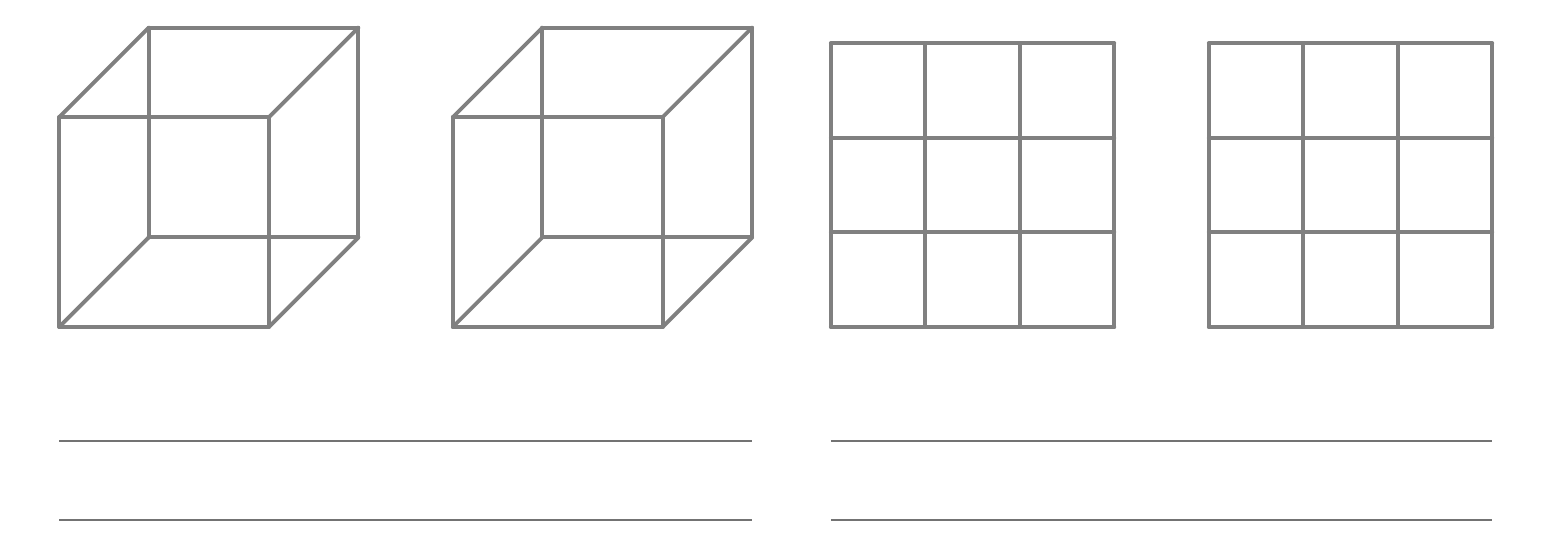
\begin{tikzpicture}
\useasboundingbox (0,0) rectangle (19.0,6.300);
\draw[stroke] (0.400,2.500) -- (3.064,2.500);
\draw[stroke] (3.064,2.500) -- (3.064,5.164);
\draw[stroke] (3.064,5.164) -- (0.400,5.164);
\draw[stroke] (0.400,5.164) -- (0.400,2.500);
\draw[stroke] (1.536,3.636) -- (4.200,3.636);
\draw[stroke] (4.200,3.636) -- (4.200,6.300);
\draw[stroke] (4.200,6.300) -- (1.536,6.300);
\draw[stroke] (1.536,6.300) -- (1.536,3.636);
\draw[stroke] (0.400,2.500) -- (1.536,3.636);
\draw[stroke] (3.064,2.500) -- (4.200,3.636);
\draw[stroke] (3.064,5.164) -- (4.200,6.300);
\draw[stroke] (0.400,5.164) -- (1.536,6.300);
\draw[stroke] (5.400,2.500) -- (8.064,2.500);
\draw[stroke] (8.064,2.500) -- (8.064,5.164);
\draw[stroke] (8.064,5.164) -- (5.400,5.164);
\draw[stroke] (5.400,5.164) -- (5.400,2.500);
\draw[stroke] (6.536,3.636) -- (9.200,3.636);
\draw[stroke] (9.200,3.636) -- (9.200,6.300);
\draw[stroke] (9.200,6.300) -- (6.536,6.300);
\draw[stroke] (6.536,6.300) -- (6.536,3.636);
\draw[stroke] (5.400,2.500) -- (6.536,3.636);
\draw[stroke] (8.064,2.500) -- (9.200,3.636);
\draw[stroke] (8.064,5.164) -- (9.200,6.300);
\draw[stroke] (5.400,5.164) -- (6.536,6.300);
\draw[black!55, line width=0.6pt] (0.400,0.050) -- ++(8.800,0);
\draw[black!55, line width=0.6pt] (0.400,1.050) -- ++(8.800,0);
\draw[stroke] (10.200,2.500) -- (10.200,6.100);
\draw[stroke] (10.200,2.500) -- (13.800,2.500);
\draw[stroke] (11.400,2.500) -- (11.400,6.100);
\draw[stroke] (10.200,3.700) -- (13.800,3.700);
\draw[stroke] (12.600,2.500) -- (12.600,6.100);
\draw[stroke] (10.200,4.900) -- (13.800,4.900);
\draw[stroke] (13.800,2.500) -- (13.800,6.100);
\draw[stroke] (10.200,6.100) -- (13.800,6.100);
\draw[stroke] (15.000,2.500) -- (15.000,6.100);
\draw[stroke] (15.000,2.500) -- (18.600,2.500);
\draw[stroke] (16.200,2.500) -- (16.200,6.100);
\draw[stroke] (15.000,3.700) -- (18.600,3.700);
\draw[stroke] (17.400,2.500) -- (17.400,6.100);
\draw[stroke] (15.000,4.900) -- (18.600,4.900);
\draw[stroke] (18.600,2.500) -- (18.600,6.100);
\draw[stroke] (15.000,6.100) -- (18.600,6.100);
\draw[black!55, line width=0.6pt] (10.200,0.050) -- ++(8.400,0);
\draw[black!55, line width=0.6pt] (10.200,1.050) -- ++(8.400,0);
\end{tikzpicture}


\par\vspace{7mm}\noindent 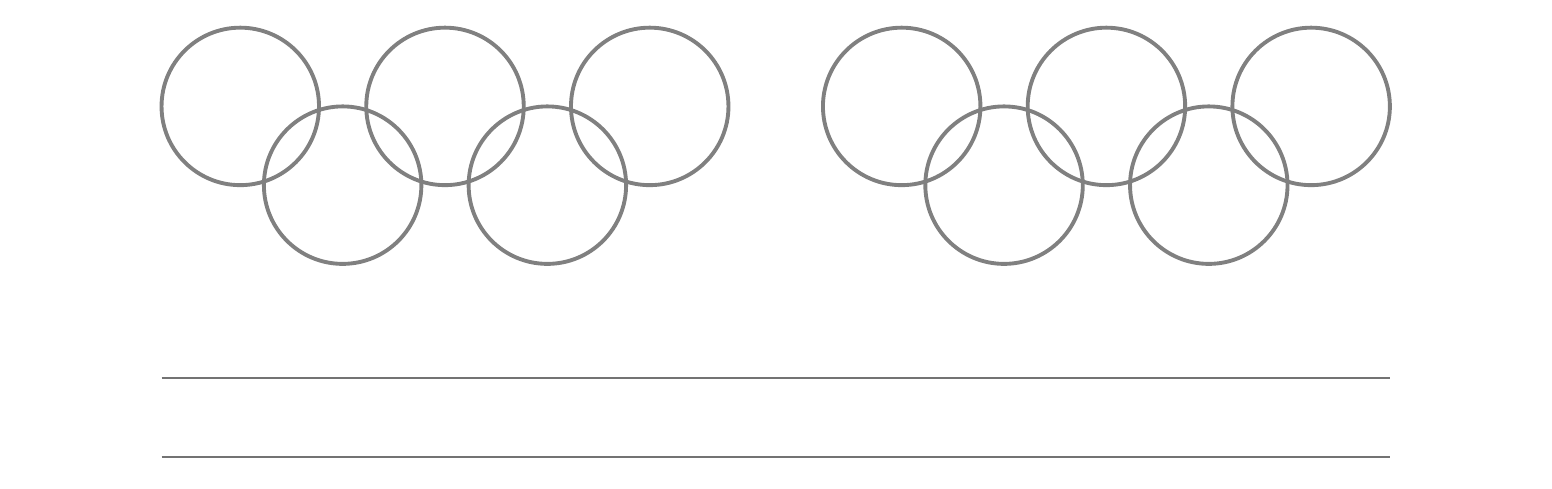
\begin{tikzpicture}
\useasboundingbox (0,0) rectangle (19.0,5.500);
\draw[stroke] (2.700,4.500) circle (1.000);
\draw[stroke] (5.300,4.500) circle (1.000);
\draw[stroke] (7.900,4.500) circle (1.000);
\draw[stroke] (4.000,3.500) circle (1.000);
\draw[stroke] (6.600,3.500) circle (1.000);
\draw[stroke] (11.100,4.500) circle (1.000);
\draw[stroke] (13.700,4.500) circle (1.000);
\draw[stroke] (16.300,4.500) circle (1.000);
\draw[stroke] (12.400,3.500) circle (1.000);
\draw[stroke] (15.000,3.500) circle (1.000);
\draw[black!55, line width=0.6pt] (1.700,0.050) -- ++(15.600,0);
\draw[black!55, line width=0.6pt] (1.700,1.050) -- ++(15.600,0);
\end{tikzpicture}


\par\vspace{7mm}\noindent 
\begin{tikzpicture}
\useasboundingbox (0,0) rectangle (19.0,5.937);
\draw[stroke] (7.000,5.937) -- (5.193,4.624);
\draw[stroke] (5.193,4.624) -- (5.883,2.500);
\draw[stroke] (5.883,2.500) -- (8.117,2.500);
\draw[stroke] (8.117,2.500) -- (8.807,4.624);
\draw[stroke] (8.807,4.624) -- (7.000,5.937);
\draw[stroke] (7.000,5.937) -- (5.883,2.500);
\draw[stroke] (5.193,4.624) -- (8.117,2.500);
\draw[stroke] (5.883,2.500) -- (8.807,4.624);
\draw[stroke] (8.117,2.500) -- (7.000,5.937);
\draw[stroke] (8.807,4.624) -- (5.193,4.624);
\draw[stroke] (12.000,5.937) -- (10.193,4.624);
\draw[stroke] (10.193,4.624) -- (10.883,2.500);
\draw[stroke] (10.883,2.500) -- (13.117,2.500);
\draw[stroke] (13.117,2.500) -- (13.807,4.624);
\draw[stroke] (13.807,4.624) -- (12.000,5.937);
\draw[stroke] (12.000,5.937) -- (10.883,2.500);
\draw[stroke] (10.193,4.624) -- (13.117,2.500);
\draw[stroke] (10.883,2.500) -- (13.807,4.624);
\draw[stroke] (13.117,2.500) -- (12.000,5.937);
\draw[stroke] (13.807,4.624) -- (10.193,4.624);
\draw[black!55, line width=0.6pt] (5.100,0.050) -- ++(8.800,0);
\draw[black!55, line width=0.6pt] (5.100,1.050) -- ++(8.800,0);
\end{tikzpicture}


\par\vspace{9mm}

\begin{minipage}{\linewidth}\raggedright
\prob{8}Lee walked around the outside of this town: \mbox{A B C D E F G H I A}. Find a walk from A back to A that crosses every bridge exactly once, and in which Lee's nine bridges still come in the order Lee crossed them.

\vspace{5mm}\noindent 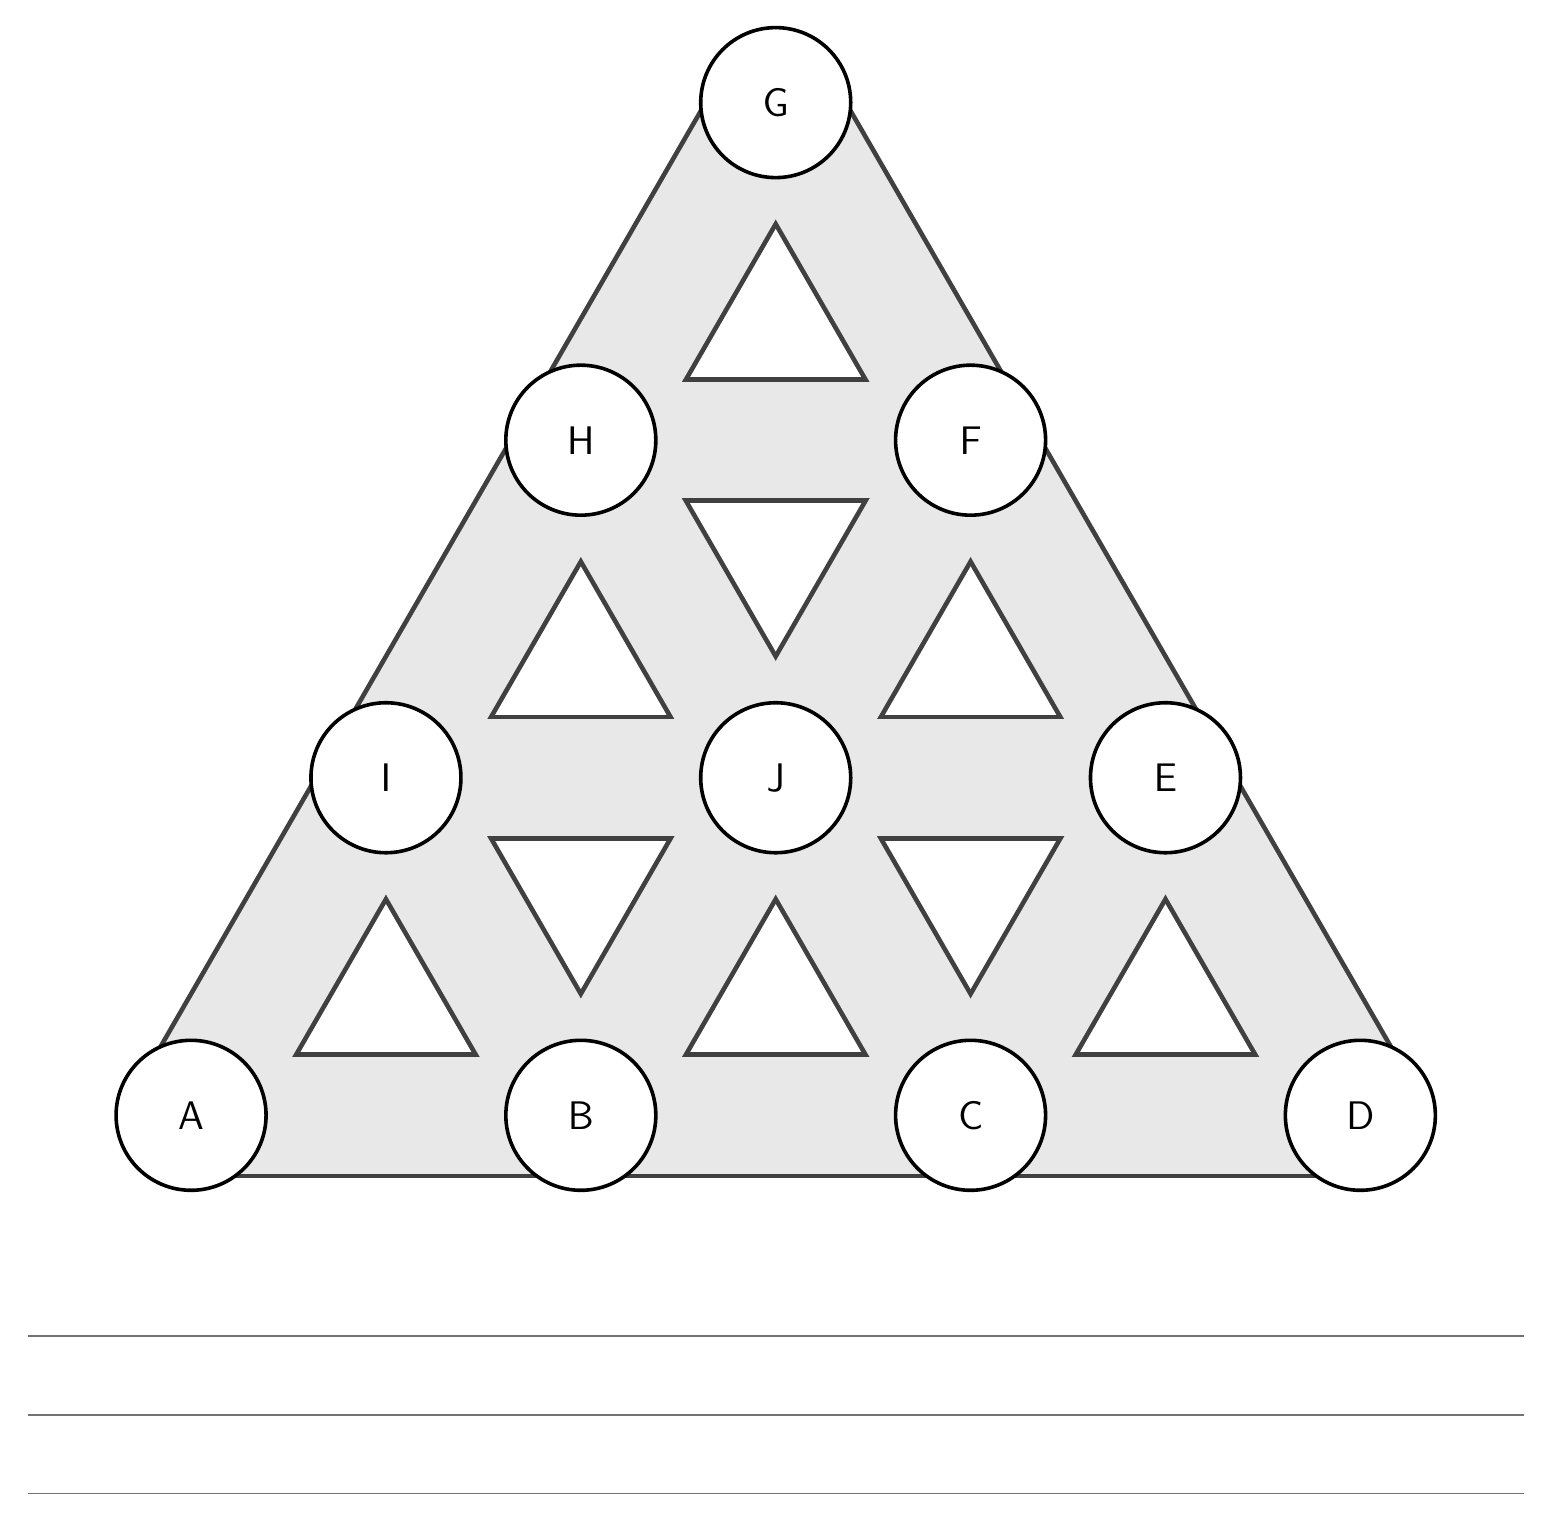
\begin{tikzpicture}
\useasboundingbox (0,0) rectangle (19.0,18.665);
\draw[bandout] (2.075,4.852) -- (7.025,4.852);
\draw[bandout] (2.075,4.852) -- (4.550,9.139);
\draw[bandout] (7.025,4.852) -- (11.975,4.852);
\draw[bandout] (7.025,4.852) -- (9.500,9.139);
\draw[bandout] (7.025,4.852) -- (4.550,9.139);
\draw[bandout] (11.975,4.852) -- (16.925,4.852);
\draw[bandout] (11.975,4.852) -- (14.450,9.139);
\draw[bandout] (11.975,4.852) -- (9.500,9.139);
\draw[bandout] (16.925,4.852) -- (14.450,9.139);
\draw[bandout] (4.550,9.139) -- (9.500,9.139);
\draw[bandout] (4.550,9.139) -- (7.025,13.426);
\draw[bandout] (9.500,9.139) -- (14.450,9.139);
\draw[bandout] (9.500,9.139) -- (11.975,13.426);
\draw[bandout] (9.500,9.139) -- (7.025,13.426);
\draw[bandout] (14.450,9.139) -- (11.975,13.426);
\draw[bandout] (7.025,13.426) -- (11.975,13.426);
\draw[bandout] (7.025,13.426) -- (9.500,17.713);
\draw[bandout] (11.975,13.426) -- (9.500,17.713);
\draw[bandfill] (2.075,4.852) -- (7.025,4.852);
\draw[bandfill] (2.075,4.852) -- (4.550,9.139);
\draw[bandfill] (7.025,4.852) -- (11.975,4.852);
\draw[bandfill] (7.025,4.852) -- (9.500,9.139);
\draw[bandfill] (7.025,4.852) -- (4.550,9.139);
\draw[bandfill] (11.975,4.852) -- (16.925,4.852);
\draw[bandfill] (11.975,4.852) -- (14.450,9.139);
\draw[bandfill] (11.975,4.852) -- (9.500,9.139);
\draw[bandfill] (16.925,4.852) -- (14.450,9.139);
\draw[bandfill] (4.550,9.139) -- (9.500,9.139);
\draw[bandfill] (4.550,9.139) -- (7.025,13.426);
\draw[bandfill] (9.500,9.139) -- (14.450,9.139);
\draw[bandfill] (9.500,9.139) -- (11.975,13.426);
\draw[bandfill] (9.500,9.139) -- (7.025,13.426);
\draw[bandfill] (14.450,9.139) -- (11.975,13.426);
\draw[bandfill] (7.025,13.426) -- (11.975,13.426);
\draw[bandfill] (7.025,13.426) -- (9.500,17.713);
\draw[bandfill] (11.975,13.426) -- (9.500,17.713);
\draw[island] (2.075,4.852) circle (0.9525);
\node[islandlabel] at (2.075,4.852) {A};
\draw[island] (7.025,4.852) circle (0.9525);
\node[islandlabel] at (7.025,4.852) {B};
\draw[island] (11.975,4.852) circle (0.9525);
\node[islandlabel] at (11.975,4.852) {C};
\draw[island] (16.925,4.852) circle (0.9525);
\node[islandlabel] at (16.925,4.852) {D};
\draw[island] (4.550,9.139) circle (0.9525);
\node[islandlabel] at (4.550,9.139) {I};
\draw[island] (9.500,9.139) circle (0.9525);
\node[islandlabel] at (9.500,9.139) {J};
\draw[island] (14.450,9.139) circle (0.9525);
\node[islandlabel] at (14.450,9.139) {E};
\draw[island] (7.025,13.426) circle (0.9525);
\node[islandlabel] at (7.025,13.426) {H};
\draw[island] (11.975,13.426) circle (0.9525);
\node[islandlabel] at (11.975,13.426) {F};
\draw[island] (9.500,17.713) circle (0.9525);
\node[islandlabel] at (9.500,17.713) {G};
\draw[black!55, line width=0.6pt] (0.000,0.050) -- ++(19.0,0);
\draw[black!55, line width=0.6pt] (0.000,1.050) -- ++(19.0,0);
\draw[black!55, line width=0.6pt] (0.000,2.050) -- ++(19.0,0);
\end{tikzpicture}
\end{minipage}


\par\vspace{9mm}

\begin{minipage}{\linewidth}\raggedright
\prob{9}Explain why a town in which every island has an even number of bridges always has a walk that crosses every bridge exactly once and ends where it started. Then explain why a town with exactly two islands that have an odd number of bridges always has a walk that crosses every bridge exactly once.

\vspace{5mm}\noindent \begin{tikzpicture}
\useasboundingbox (0,0) rectangle (19.0,7.000);
\draw[black!55, line width=0.6pt] (0.000,0.050) -- ++(19.0,0);
\draw[black!55, line width=0.6pt] (0.000,1.050) -- ++(19.0,0);
\draw[black!55, line width=0.6pt] (0.000,2.050) -- ++(19.0,0);
\draw[black!55, line width=0.6pt] (0.000,3.050) -- ++(19.0,0);
\draw[black!55, line width=0.6pt] (0.000,4.050) -- ++(19.0,0);
\draw[black!55, line width=0.6pt] (0.000,5.050) -- ++(19.0,0);
\draw[black!55, line width=0.6pt] (0.000,6.050) -- ++(19.0,0);
\end{tikzpicture}
\end{minipage}


\par\vspace{9mm}

\newpage

\begin{minipage}{\linewidth}\raggedright
\prob{10}A truck must cross every bridge of a town at least once. Before it starts, you may put extra counters on bridges, and a bridge with two counters is crossed two times. For each town, find the fewest extra counters for a route that ends where it started, and the fewest for a route that may end anywhere.

\vspace{5mm}\noindent 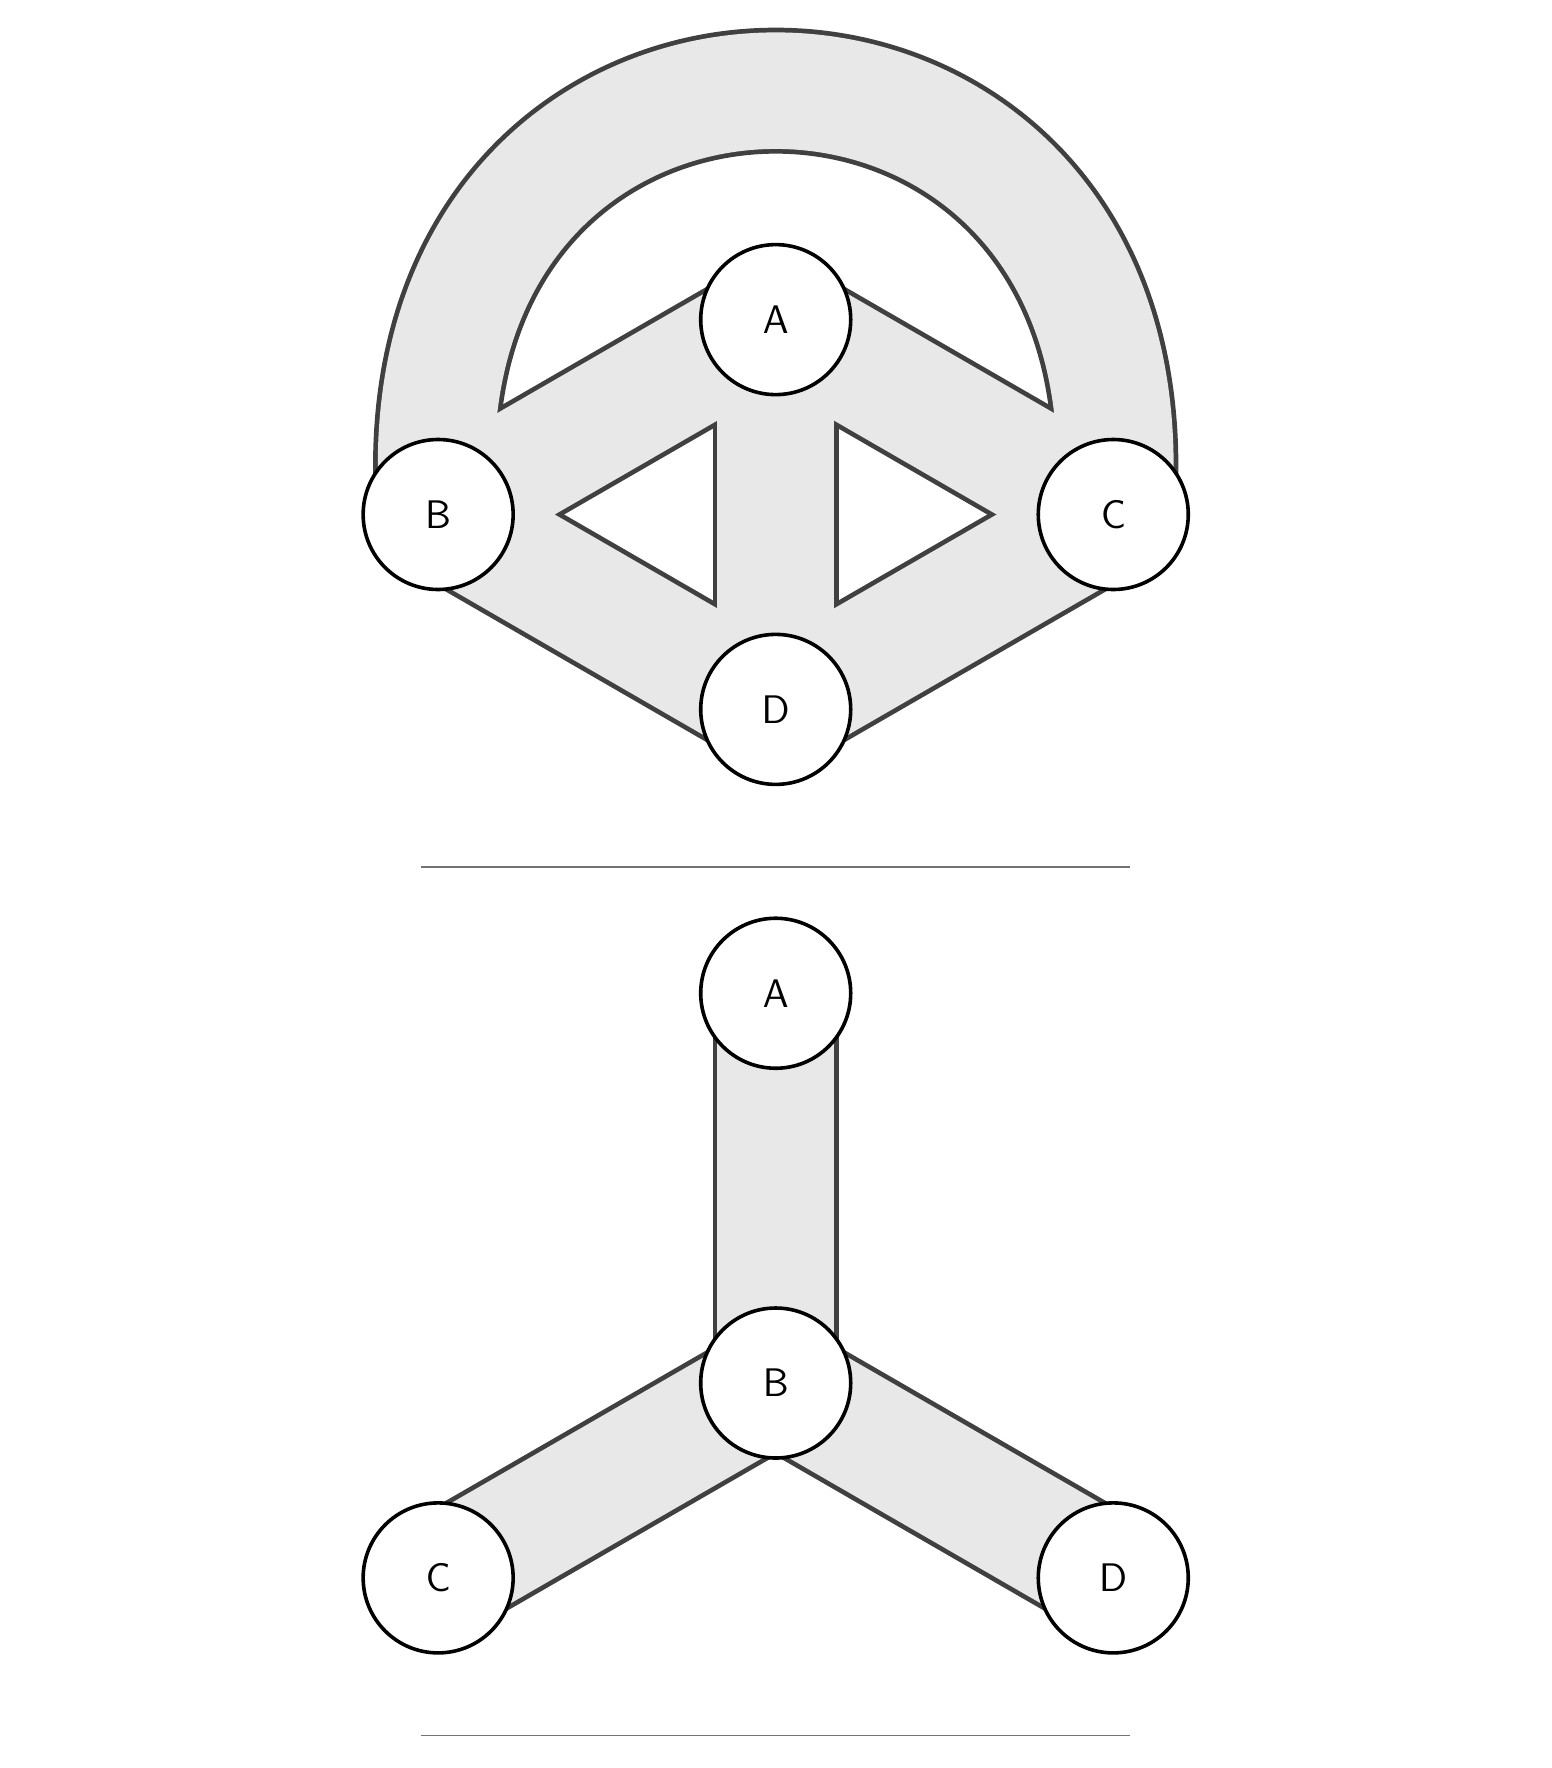
\begin{tikzpicture}
\useasboundingbox (0,0) rectangle (19.0,21.741);
\draw[bandout] (9.500,18.033) -- (9.500,13.083);
\draw[bandout] (9.500,18.033) -- (5.213,15.558);
\draw[bandout] (9.500,18.033) -- (13.787,15.558);
\draw[bandout] (9.500,13.083) -- (5.213,15.558);
\draw[bandout] (9.500,13.083) -- (13.787,15.558);
\draw[bandout] (5.213,15.558) .. controls (4.613,22.735) and (14.387,22.735) .. (13.787,15.558);
\draw[bandfill] (9.500,18.033) -- (9.500,13.083);
\draw[bandfill] (9.500,18.033) -- (5.213,15.558);
\draw[bandfill] (9.500,18.033) -- (13.787,15.558);
\draw[bandfill] (9.500,13.083) -- (5.213,15.558);
\draw[bandfill] (9.500,13.083) -- (13.787,15.558);
\draw[bandfill] (5.213,15.558) .. controls (4.613,22.735) and (14.387,22.735) .. (13.787,15.558);
\draw[island] (9.500,18.033) circle (0.9525);
\node[islandlabel] at (9.500,18.033) {A};
\draw[island] (9.500,13.083) circle (0.9525);
\node[islandlabel] at (9.500,13.083) {D};
\draw[island] (5.213,15.558) circle (0.9525);
\node[islandlabel] at (5.213,15.558) {B};
\draw[island] (13.787,15.558) circle (0.9525);
\node[islandlabel] at (13.787,15.558) {C};
\draw[black!55, line width=0.6pt] (5.000,11.080) -- ++(9.0,0);
\draw[bandout] (9.500,4.528) -- (9.500,9.478);
\draw[bandout] (9.500,4.528) -- (5.213,2.053);
\draw[bandout] (9.500,4.528) -- (13.787,2.053);
\draw[bandfill] (9.500,4.528) -- (9.500,9.478);
\draw[bandfill] (9.500,4.528) -- (5.213,2.053);
\draw[bandfill] (9.500,4.528) -- (13.787,2.053);
\draw[island] (9.500,4.528) circle (0.9525);
\node[islandlabel] at (9.500,4.528) {B};
\draw[island] (9.500,9.478) circle (0.9525);
\node[islandlabel] at (9.500,9.478) {A};
\draw[island] (5.213,2.053) circle (0.9525);
\node[islandlabel] at (5.213,2.053) {C};
\draw[island] (13.787,2.053) circle (0.9525);
\node[islandlabel] at (13.787,2.053) {D};
\draw[black!55, line width=0.6pt] (5.000,0.050) -- ++(9.0,0);
\end{tikzpicture}
\end{minipage}


\par\vspace{7mm}\noindent 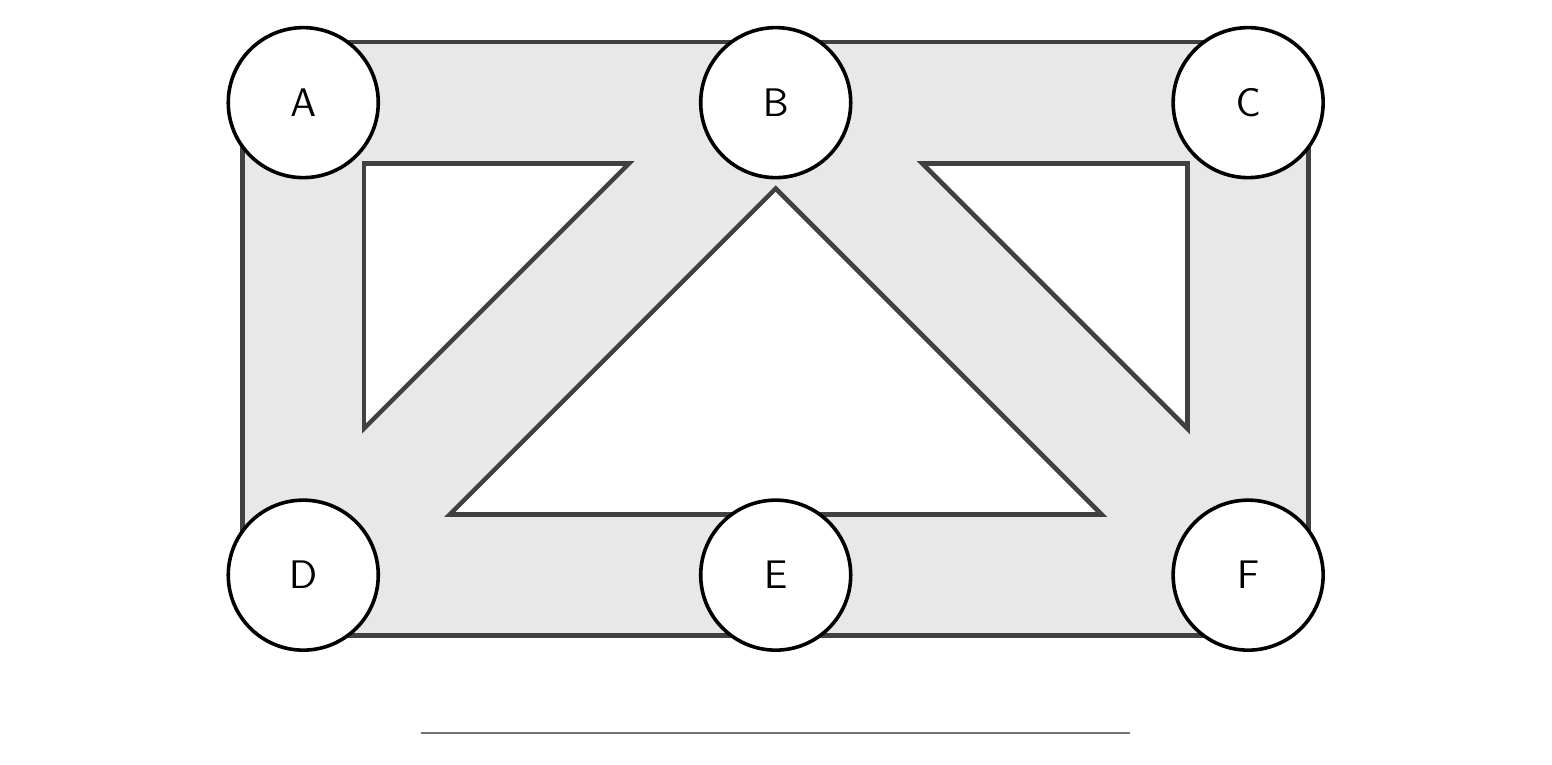
\begin{tikzpicture}
\useasboundingbox (0,0) rectangle (19.0,9.005);
\draw[bandout] (3.500,2.052) -- (9.500,2.052);
\draw[bandout] (9.500,2.052) -- (15.500,2.052);
\draw[bandout] (3.500,8.053) -- (9.500,8.053);
\draw[bandout] (9.500,8.053) -- (15.500,8.053);
\draw[bandout] (3.500,2.052) -- (3.500,8.053);
\draw[bandout] (15.500,2.052) -- (15.500,8.053);
\draw[bandout] (9.500,8.053) -- (3.500,2.052);
\draw[bandout] (9.500,8.053) -- (15.500,2.052);
\draw[bandfill] (3.500,2.052) -- (9.500,2.052);
\draw[bandfill] (9.500,2.052) -- (15.500,2.052);
\draw[bandfill] (3.500,8.053) -- (9.500,8.053);
\draw[bandfill] (9.500,8.053) -- (15.500,8.053);
\draw[bandfill] (3.500,2.052) -- (3.500,8.053);
\draw[bandfill] (15.500,2.052) -- (15.500,8.053);
\draw[bandfill] (9.500,8.053) -- (3.500,2.052);
\draw[bandfill] (9.500,8.053) -- (15.500,2.052);
\draw[island] (3.500,2.052) circle (0.9525);
\node[islandlabel] at (3.500,2.052) {D};
\draw[island] (3.500,8.053) circle (0.9525);
\node[islandlabel] at (3.500,8.053) {A};
\draw[island] (9.500,2.052) circle (0.9525);
\node[islandlabel] at (9.500,2.052) {E};
\draw[island] (9.500,8.053) circle (0.9525);
\node[islandlabel] at (9.500,8.053) {B};
\draw[island] (15.500,2.052) circle (0.9525);
\node[islandlabel] at (15.500,2.052) {F};
\draw[island] (15.500,8.053) circle (0.9525);
\node[islandlabel] at (15.500,8.053) {C};
\draw[black!55, line width=0.6pt] (5.000,0.050) -- ++(9.0,0);
\end{tikzpicture}


\par\vspace{9mm}

\begin{minipage}{\linewidth}\raggedright
\prob{11}In the first town of Problem 10, explain why no route that ends where it started can use fewer extra counters than your answer.

\vspace{5mm}\noindent \begin{tikzpicture}
\useasboundingbox (0,0) rectangle (19.0,6.000);
\draw[black!55, line width=0.6pt] (0.000,0.050) -- ++(19.0,0);
\draw[black!55, line width=0.6pt] (0.000,1.050) -- ++(19.0,0);
\draw[black!55, line width=0.6pt] (0.000,2.050) -- ++(19.0,0);
\draw[black!55, line width=0.6pt] (0.000,3.050) -- ++(19.0,0);
\draw[black!55, line width=0.6pt] (0.000,4.050) -- ++(19.0,0);
\draw[black!55, line width=0.6pt] (0.000,5.050) -- ++(19.0,0);
\end{tikzpicture}
\end{minipage}


\par\vspace{9mm}
\end{document}
